%%%%%%%%%%%%%%%%%%%%%%%%%%%%%%%%%%%%%%%%%
% Lachaise Assignment
% LaTeX Template
% Version 1.0 (26/6/2018)
%
% This template originates from:
% http://www.LaTeXTemplates.com
%
% Authors:
% Marion Lachaise & François Févotte
% Vel (vel@LaTeXTemplates.com)
%
% License:
% CC BY-NC-SA 3.0 (http://creativecommons.org/licenses/by-nc-sa/3.0/)
% 
%%%%%%%%%%%%%%%%%%%%%%%%%%%%%%%%%%%%%%%%%

%----------------------------------------------------------------------------------------
%	PACKAGES AND OTHER DOCUMENT CONFIGURATIONS
%----------------------------------------------------------------------------------------

\documentclass[12pt]{article}
\usepackage{graphicx}
\usepackage{amsmath}
\usepackage{fontawesome5}
\usepackage{booktabs}
\usepackage{amssymb}
\usepackage{hyperref}
\usepackage{amsthm}
\usepackage{newpxtext}
\usepackage[toc,page]{appendix}
\usepackage[nottoc]{tocbibind}
\numberwithin{equation}{section}
\graphicspath{ {./Images/} }
\usepackage[raggedright]{titlesec}
%%%%%%%%%%%%%%%%%%%%%%%%%%%%%%%%%%%%%%%%%
% Lachaise Assignment
% Structure Specification File
% Version 1.0 (26/6/2018)
%
% This template originates from:
% http://www.LaTeXTemplates.com
%
% Authors:
% Marion Lachaise & François Févotte
% Vel (vel@LaTeXTemplates.com)
%
% License:
% CC BY-NC-SA 3.0 (http://creativecommons.org/licenses/by-nc-sa/3.0/)
% 
%%%%%%%%%%%%%%%%%%%%%%%%%%%%%%%%%%%%%%%%%

%----------------------------------------------------------------------------------------
%	PACKAGES AND OTHER DOCUMENT CONFIGURATIONS
%----------------------------------------------------------------------------------------

\usepackage{amsmath,amsfonts,stmaryrd,amssymb} % Math packages

\usepackage{enumerate} % Custom item numbers for enumerations

\usepackage[ruled]{algorithm2e} % Algorithms

\usepackage[framemethod=tikz]{mdframed} % Allows defining custom boxed/framed environments

\usepackage{listings} % File listings, with syntax highlighting
\lstset{
	basicstyle=\ttfamily, % Typeset listings in monospace font
}

%----------------------------------------------------------------------------------------
%	DOCUMENT MARGINS
%----------------------------------------------------------------------------------------

\usepackage{geometry} % Required for adjusting page dimensions and margins

\geometry{
	paper=a4paper, % Paper size, change to letterpaper for US letter size
	top=3.81cm, % Top margin
	bottom=3.81cm, % Bottom margin
	left=3.81cm, % Left margin
	right=3.81cm, % Right margin
	headheight=14pt, % Header height
	footskip=1.5cm, % Space from the bottom margin to the baseline of the footer
	headsep=1.2cm, % Space from the top margin to the baseline of the header
	%showframe, % Uncomment to show how the type block is set on the page
}

%----------------------------------------------------------------------------------------
%	FONTS
%----------------------------------------------------------------------------------------

\usepackage[utf8]{inputenc} % Required for inputting international characters
\usepackage[T1]{fontenc} % Output font encoding for international characters

 % Use the XCharter fonts

%----------------------------------------------------------------------------------------
%	COMMAND LINE ENVIRONMENT
%----------------------------------------------------------------------------------------

% Usage:
% \begin{commandline}
%	\begin{verbatim}
%		$ ls
%		
%		Applications	Desktop	...
%	\end{verbatim}
% \end{commandline}

\mdfdefinestyle{commandline}{
	leftmargin=10pt,
	rightmargin=10pt,
	innerleftmargin=15pt,
	middlelinecolor=black!50!white,
	middlelinewidth=2pt,
	frametitlerule=false,
	backgroundcolor=black!5!white,
	frametitle={Command Line},
	frametitlefont={\normalfont\sffamily\color{white}\hspace{-1em}},
	frametitlebackgroundcolor=black!50!white,
	nobreak,
}

% Define a custom environment for command-line snapshots
\newenvironment{commandline}{
	\medskip
	\begin{mdframed}[style=commandline]
}{
	\end{mdframed}
	\medskip
}

%----------------------------------------------------------------------------------------
%	FILE CONTENTS ENVIRONMENT
%----------------------------------------------------------------------------------------

% Usage:
% \begin{file}[optional filename, defaults to "File"]
%	File contents, for example, with a listings environment
% \end{file}

\mdfdefinestyle{file}{
	innertopmargin=1.6\baselineskip,
	innerbottommargin=0.8\baselineskip,
	topline=false, bottomline=false,
	leftline=false, rightline=false,
	leftmargin=2cm,
	rightmargin=2cm,
	singleextra={%
		\draw[fill=black!10!white](P)++(0,-1.2em)rectangle(P-|O);
		\node[anchor=north west]
		at(P-|O){\ttfamily\mdfilename};
		%
		\def\l{3em}
		\draw(O-|P)++(-\l,0)--++(\l,\l)--(P)--(P-|O)--(O)--cycle;
		\draw(O-|P)++(-\l,0)--++(0,\l)--++(\l,0);
	},
	nobreak,
}

% Define a custom environment for file contents
\newenvironment{file}[1][File]{ % Set the default filename to "File"
	\medskip
	\newcommand{\mdfilename}{#1}
	\begin{mdframed}[style=file]
}{
	\end{mdframed}
	\medskip
}

%----------------------------------------------------------------------------------------
%	NUMBERED QUESTIONS ENVIRONMENT
%----------------------------------------------------------------------------------------

% Usage:
% \begin{question}[optional title]
% Question contents
% \end{question}

\mdfdefinestyle{question}{
	innertopmargin=1.2\baselineskip,
	innerbottommargin=0.8\baselineskip,
	roundcorner=5pt,
	nobreak,
	singleextra={%
		\draw(P-|O)node[xshift=1em,anchor=west,fill=white,draw,rounded corners=5pt]{%
		\theQuestion\questionTitle};
	},
}


% Define a custom environment for numbered questions
\newenvironment{question}[1][\unskip]{
	\bigskip
	\stepcounter{Question}
	\newcommand{\questionTitle}{~#1}
	\begin{mdframed}[style=question]
}{
	\end{mdframed}
	\medskip
}

%----------------------------------------------------------------------------------------
%	WARNING TEXT ENVIRONMENT
%----------------------------------------------------------------------------------------

% Usage:
% \begin{warn}[optional title, defaults to "Warning:"]
%	Contents
% \end{warn}

\mdfdefinestyle{warning}{
	topline=false, bottomline=false,
	leftline=false, rightline=false,
	nobreak,
	singleextra={%
		\draw(P-|O)++(-0.7em,0)node(tmp1){};
		\draw(P-|O)++(0.7em,0)node(tmp2){};
		\fill[white,rotate around={45:(P-|O)}](tmp1)rectangle(tmp2);
		\node at(P-|O){\color{black}\scriptsize\bf};
		\draw[very thick](P-|O)++(0,-1em)--(O);%--(O-|P);
	}
}

% Define a custom environment for warning text
\newenvironment{warn}[1][Warning:]{ % Set the default warning to "Warning:"
	\medskip
	\begin{mdframed}[style=warning]
		\noindent{\textbf{#1}}
}{
	\end{mdframed}
}

%----------------------------------------------------------------------------------------
%	INFORMATION ENVIRONMENT
%----------------------------------------------------------------------------------------

% Usage:
% \begin{info}[optional title, defaults to "Info:"]
% 	contents
% 	\end{info}

\mdfdefinestyle{info}{%
	topline=false, bottomline=false,
	leftline=false, rightline=false,
	nobreak,
	singleextra={%
		\fill[black](P-|O)circle[radius=0.4em];
		\node at(P-|O){\color{white}\scriptsize\bf i};
		\draw[very thick](P-|O)++(0,-0.8em)--(O);%--(O-|P);
	}
}

% Define a custom environment for information
\newenvironment{info}[1][Info:]{ % Set the default title to "Info:"
	\medskip
	\begin{mdframed}[style=info]
		\noindent{\textbf{#1}}
}{
	\end{mdframed}
}
\newcommand\specpar[1]{%
  \edef\svparindent{\the\parindent}%
  \setbox0=\hbox{\parbox[t]{\dimexpr\textwidth-6pt}{\strut\hspace{\svparindent}#1\strut}}%
  \par%
  \noindent\textcolor{gray}{\rule[-\dp0]{2pt}{\dimexpr\dp0+\ht0}}\kern4pt\copy0%
  \par%
}

\newcommand{\QED}{\tag*{$\square$}}
\newtheorem{theorem}{Theorem}[section]
\newtheorem{corollary}{Corollary}[theorem]
\newtheorem{lemma}[theorem]{Lemma}
\makeatletter

\newcommand\frontmatter{%
    \cleardoublepage
  %\@mainmatterfalse
  \pagenumbering{roman}}

\newcommand\mainmatter{%
    \cleardoublepage
 % \@mainmattertrue
  \pagenumbering{arabic}}


\makeatother

\title{A look at Reciprocal\\ Multifactorial Constants}

\author{Bhoris Dhanjal}

\date{\today} 
\newcommand{\reporttitle}{{A Look at Reciprocal}\\[0.1in] {Multifactorial Constants}}


%----------------------------------------------------------------------------------------

\begin{document}
% Last modification: 2015-08-17 (Marc Deisenroth)
\begin{titlepage}

\newcommand{\HRule}{\rule{\linewidth}{0.5mm}} % Defines a new command for the horizontal lines, change thickness here




\center % Center remainder of the page

%----------------------------------------------------------------------------------------
%	HEADING SECTIONS
%----------------------------------------------------------------------------------------
\begin{center}
    



%----------------------------------------------------------------------------------------
%	TITLE SECTION
%----------------------------------------------------------------------------------------

\includegraphics[width=0.2\textwidth]{Images/xavierslogo.png}\\[1.5cm]
\HRule \\[0.4cm]
{ \huge \bfseries \reporttitle}\\[0.4cm] % Title of your document
\HRule \\[2.5cm]
\end{center}
%----------------------------------------------------------------------------------------
%	AUTHOR SECTION
%----------------------------------------------------------------------------------------
\textbf{
\large A project submitted to\\
\large Department of Mathematics\\
\large St. Xavier’s College (Autonomous), Mumbai\\
\large by\\[1cm]
\large Bhoris Dhanjal}

%----------------------------------------------------------------------------------------
%	FOOTER & DATE SECTION
%----------------------------------------------------------------------------------------
\vfill % Fill the rest of the page with whitespace
\textbf{
2020-2021}
\end{titlepage}

\frontmatter
\begin{center}
    \large St. Xavier’s College (Autonomous), Mumbai\\
\large Department of Mathematics\\
\large Project by\\
\begin{table}[h!]
\centering
\begin{tabular}{ccccc}
\hline
Sr. No. & Name of Student & Class & UID & Roll No. \\ \hline
1 & Bhoris Dhanjal & FYBSc & 202020 & 462 \\ \hline
\end{tabular}
\end{table}
Title of the Project:\\
A look at Reciprocal Multifactorial Constants
\end{center}
\clearpage

\section*{\centering{Declaration by the Student}}
\addcontentsline{toc}{section}{Declaration by the Student}
\par I hereby declare that the project entitled “A look at Reciprocal Multifactorial Constants” was completed and
written by me is the result of original project work and has not formed earlier the basis for
the certificate (any award) or similar title of this or any other school/college or examining
body.
\vfill
Date: \today \par
Name and Signature of Student:\\
\par Bhoris Dhanjal
\clearpage

\section*{\centering{Acknowledgements}}
\addcontentsline{toc}{section}{Acknowledgements}
I would like to express my deepest gratitude to my professor Dr. Ashok Bingi and the rest of the Department of Mathematics at St. Xavier's College, for giving me the wonderful chance to work on this project. Writing it has been a fantastic learning opportunity.
\par I would also like to express my special thanks towards all my friends and family that provided me with great emotional support, and helped me in proof reading my drafts.
\par I also extend my gratitude towards the vast trove of information I learnt from the internet and numerous online forums on StackExchange (Mathematics, Mathematica \& TeX).
\clearpage

\section*{\centering{Discussion on the Topic Choice}}
\addcontentsline{toc}{section}{Discussion on the Topic Choice}
Here I will discuss briefly a few important points. 
\begin{itemize}
    \item Why I choose this topic
    \item Statement of the problem
    \item Review of the relevant literature
\end{itemize}
\par The topic on Reciprocal Multifactorial Constants was chosen out of simple interest in it, and more importantly because there appeared to be no relevant mathematical literature surrounding or exploring the concepts of Reciprocal Multifactorial Constants at all. Nor were there any online sources. With the exception of, a statement of the closed form formula on Wolfram Mathworld \cite{RMFCwolfram} without any proof.
\par Hence, the original problem statement was "To prove the closed form formula for Reciprocal Multifactorial Constants". The scope of the project has since expanded.
\par The complete and detailed objectives of the project can be read in the introduction section.
\clearpage
\tableofcontents


%----------------------------------------------------------------------------------------
%	INTRODUCTION
%----------------------------------------------------------------------------------------
\mainmatter
\maketitle
\section{Introduction} % Unnumbered section
In this project we will explore the Reciprocal Multifactorial Constants (RMFC's).
The objectives of this project are as follows:
\begin{itemize}
    \item Motivating and then defining the concept of a 'multifactorial'.
    \item Defining a reciprocal multifactorial series, and displaying the convergent nature for a few examples computationally.
    \item Simply stating some of the definitions and relationships necessary for proving the closed form formula for RMFCs.
    \item Providing a proof for the closed form formula for RMFCs.
    \item Computing examples of RMFCs using both the original definition and the closed form to showcase equality between the two.
    \item Exploring computational efficiency between the series definition and the closed form definition for RMFCs.
    \item Explaining why the Reciprocal Multifactorial Series will tend to diverge as multifactorial order approaches infinity. 
    \item Exploring the asymptotics and providing two asymptotic approximations of the RMFCs.
    \item Computing absolute errors of RMFCs using the asymptotic approximations.
    \item Proving a closed form formula for Generalized RMFCs.
\end{itemize}\par
The Mathematica notebook (comprising of all code used for computations and plots) and \LaTeX \ source code can be viewed at my GitHub with the following link\\
\href{https://github.com/BhorisDhanjal/reciprocal-multifactorial-constants}{\faGithubSquare} \href{https://github.com/BhorisDhanjal/reciprocral-multifactorial-constants}{https://github.com/BhorisDhanjal/reciprocal-multifactorial-constants}
\vfill


%----------------------------------------------------------------------------------------
%	Section 2
%----------------------------------------------------------------------------------------

\section{Multifactorial} % Numbered section

To begin talking about Reciprocal Multifactorial Series  we must first clearly define the word 'multifactorial'.\par
We will denote the $k^{th}$ order multifactorial for $n \in \mathbb{N}_0$  by either $n!_{(k)}$, or using the more common notation $n\underbrace{!\ldots!}_{\text{k times}}$.

%------------------------------------------------

\subsection{Physical Intuition}
We will begin by motivating the definition of a multifactorial by giving a few examples of its occurrence.\par
For the trivial case of the first Multifactorial i.e. simply the factorial, we know of the most common example to be that $n!$ represents the total number of permutations for $n$ distinct objects.
\begin{figure}[htp]
    \centering
    $\begin{matrix}
\textup{ABCD} & \textup{BACD} & \textup{CABD} & \textup{ACBD}\\ 
\textup{BCAD} & \textup{CBAD} & \textup{CBDA} & \textup{BCDA}\\ 
\textup{DCBA }& \textup{CDBA }& \textup{BDCA }& \textup{DBCA}\\ 
\textup{DACB }& \textup{ADCB }& \textup{CDAB }& \textup{DCAB}\\ 
\textup{ACDB }& \textup{CADB }& \textup{BADC }& \textup{ABDC}\\ 
\textup{DBAC }& \textup{BDAC }& \textup{ADBC }& \textup{DABC}
\end{matrix}$
    \caption{24 permutations of 4 Objects}
    \label{fig:permutations}
\end{figure}
\par
Let us see two non-trivial examples.
\begin{itemize}
\item The number of edges without common vertices which cover every vertex of a complete graph with 2n vertices is given by the double factorial $(2n-1)!_{(2)}$ or $(2n-1)!!$. Stated in brief, the number of perfect matchings for a complete graph $K_{2n}$ is equal to $(2n-1)!!$.\par
\item Another interesting occurrence of the double factorial is in Stirling permutations. Stirling permutations of $n^{th}$ order are defined as the permutations of the multiset $\{1, 1, 2, 2, \dots n, n\}$, such that for each set of two values of $i$, the value $j$ in between the two $i$'s is greater than $i$.\par
The number of Stirling permutations for $n$ is given by the double factorial $(2n-1)!_{(2)}$ or $(2n-1)!!$.\par
\end{itemize}
For further examples refer to \textit{A combinatorial survey of identities for the double factorial} \cite{callan2009combinatorial}. Below are a few visualizations of the above discussed examples.

\begin{figure}[!htb]
    \centering
    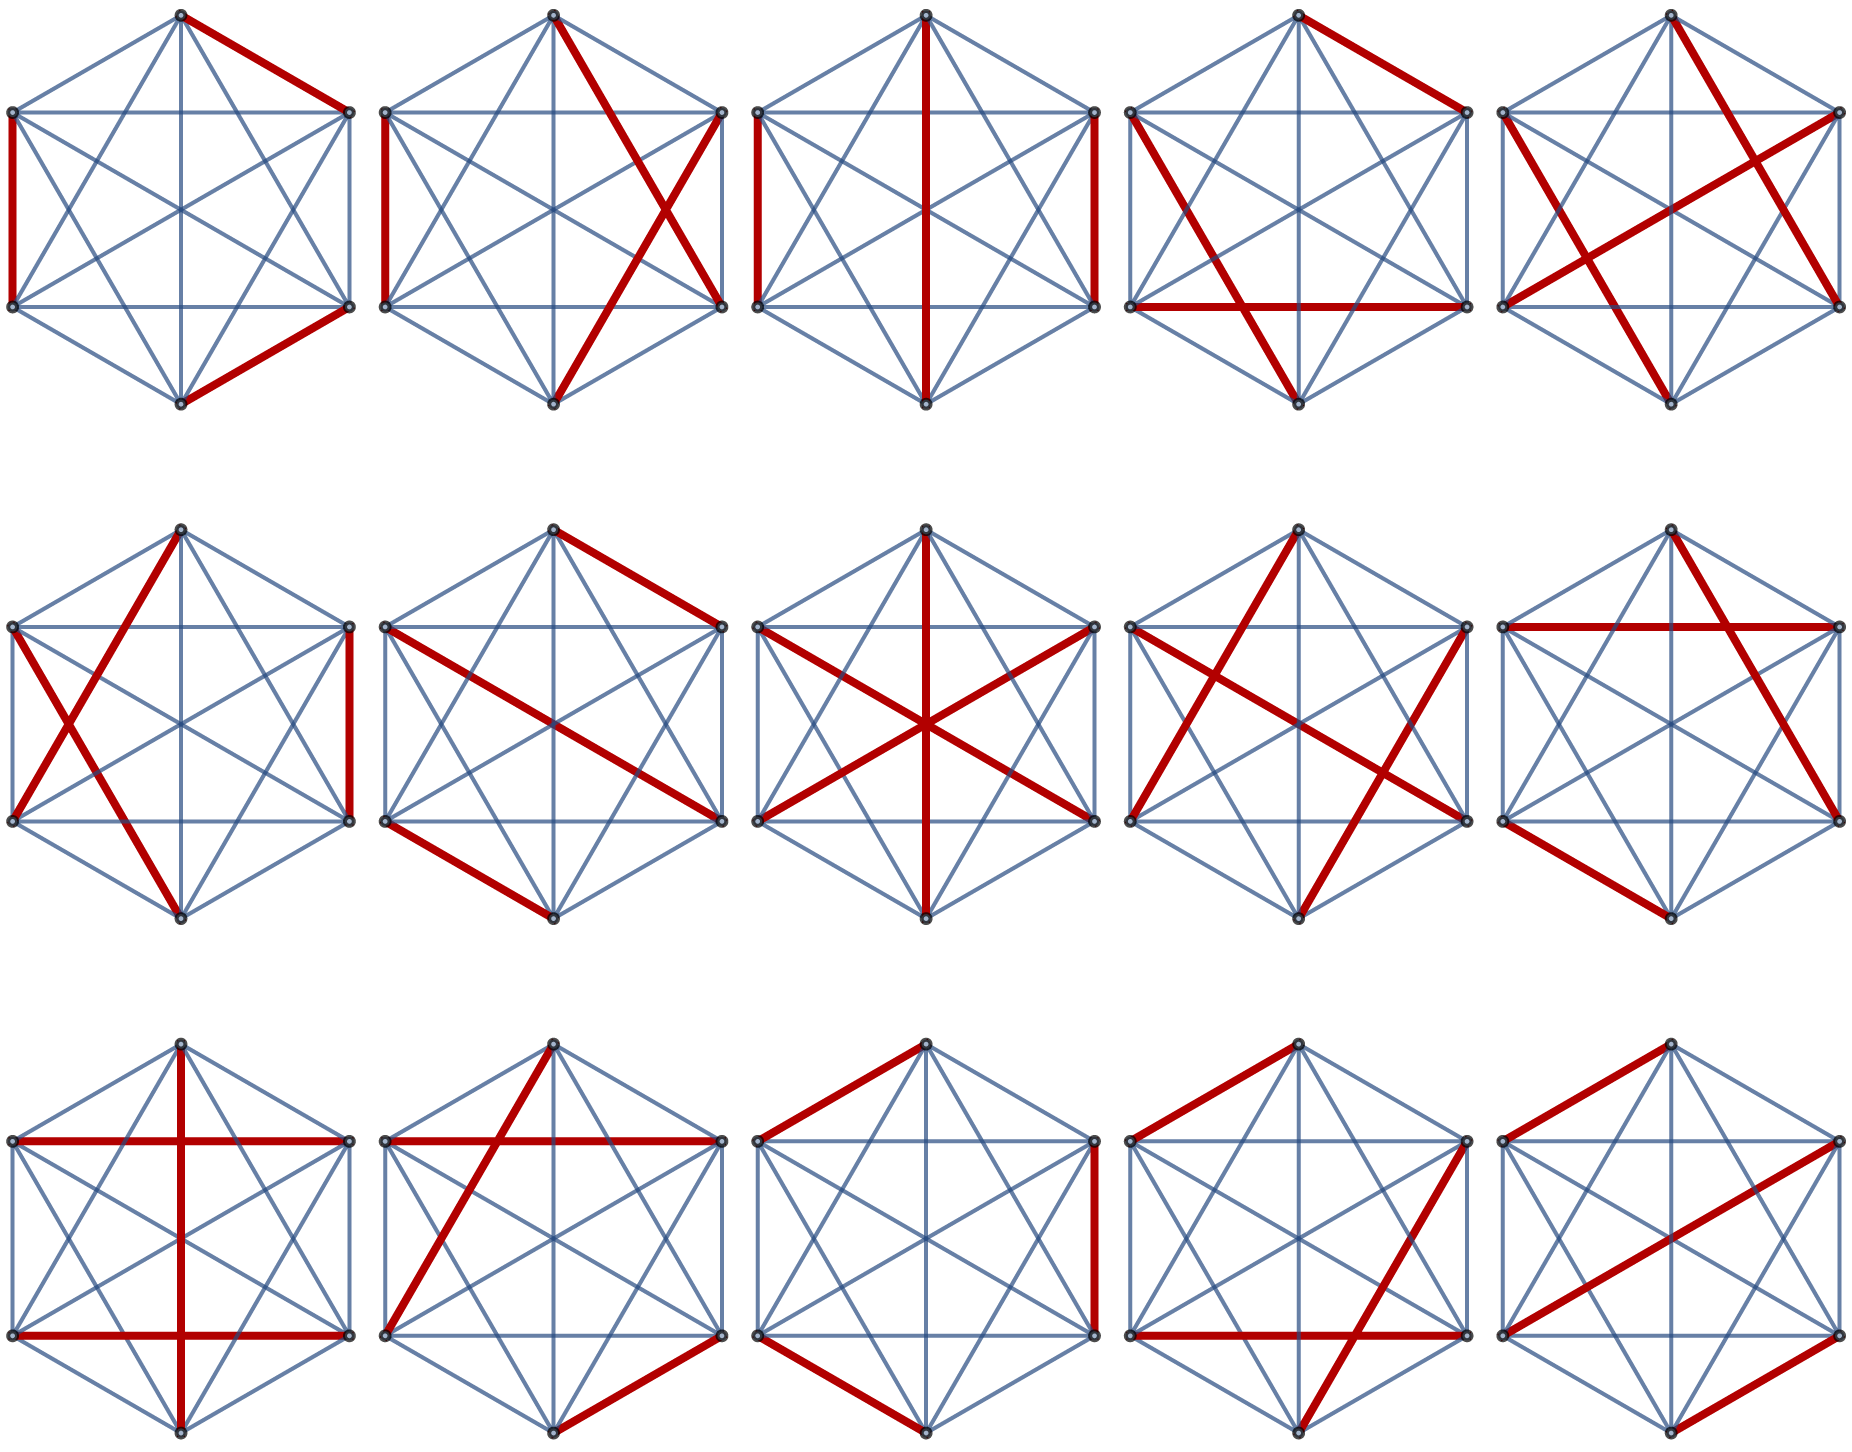
\includegraphics[width=7cm]{Images/k6matching.png}
    \caption{$(2\cdot3-1)!!=5!!=15$ perfect matchings for $K_{6}$}
    \label{fig:k6matching}
\end{figure}
\begin{figure}[!htb]
    \centering
    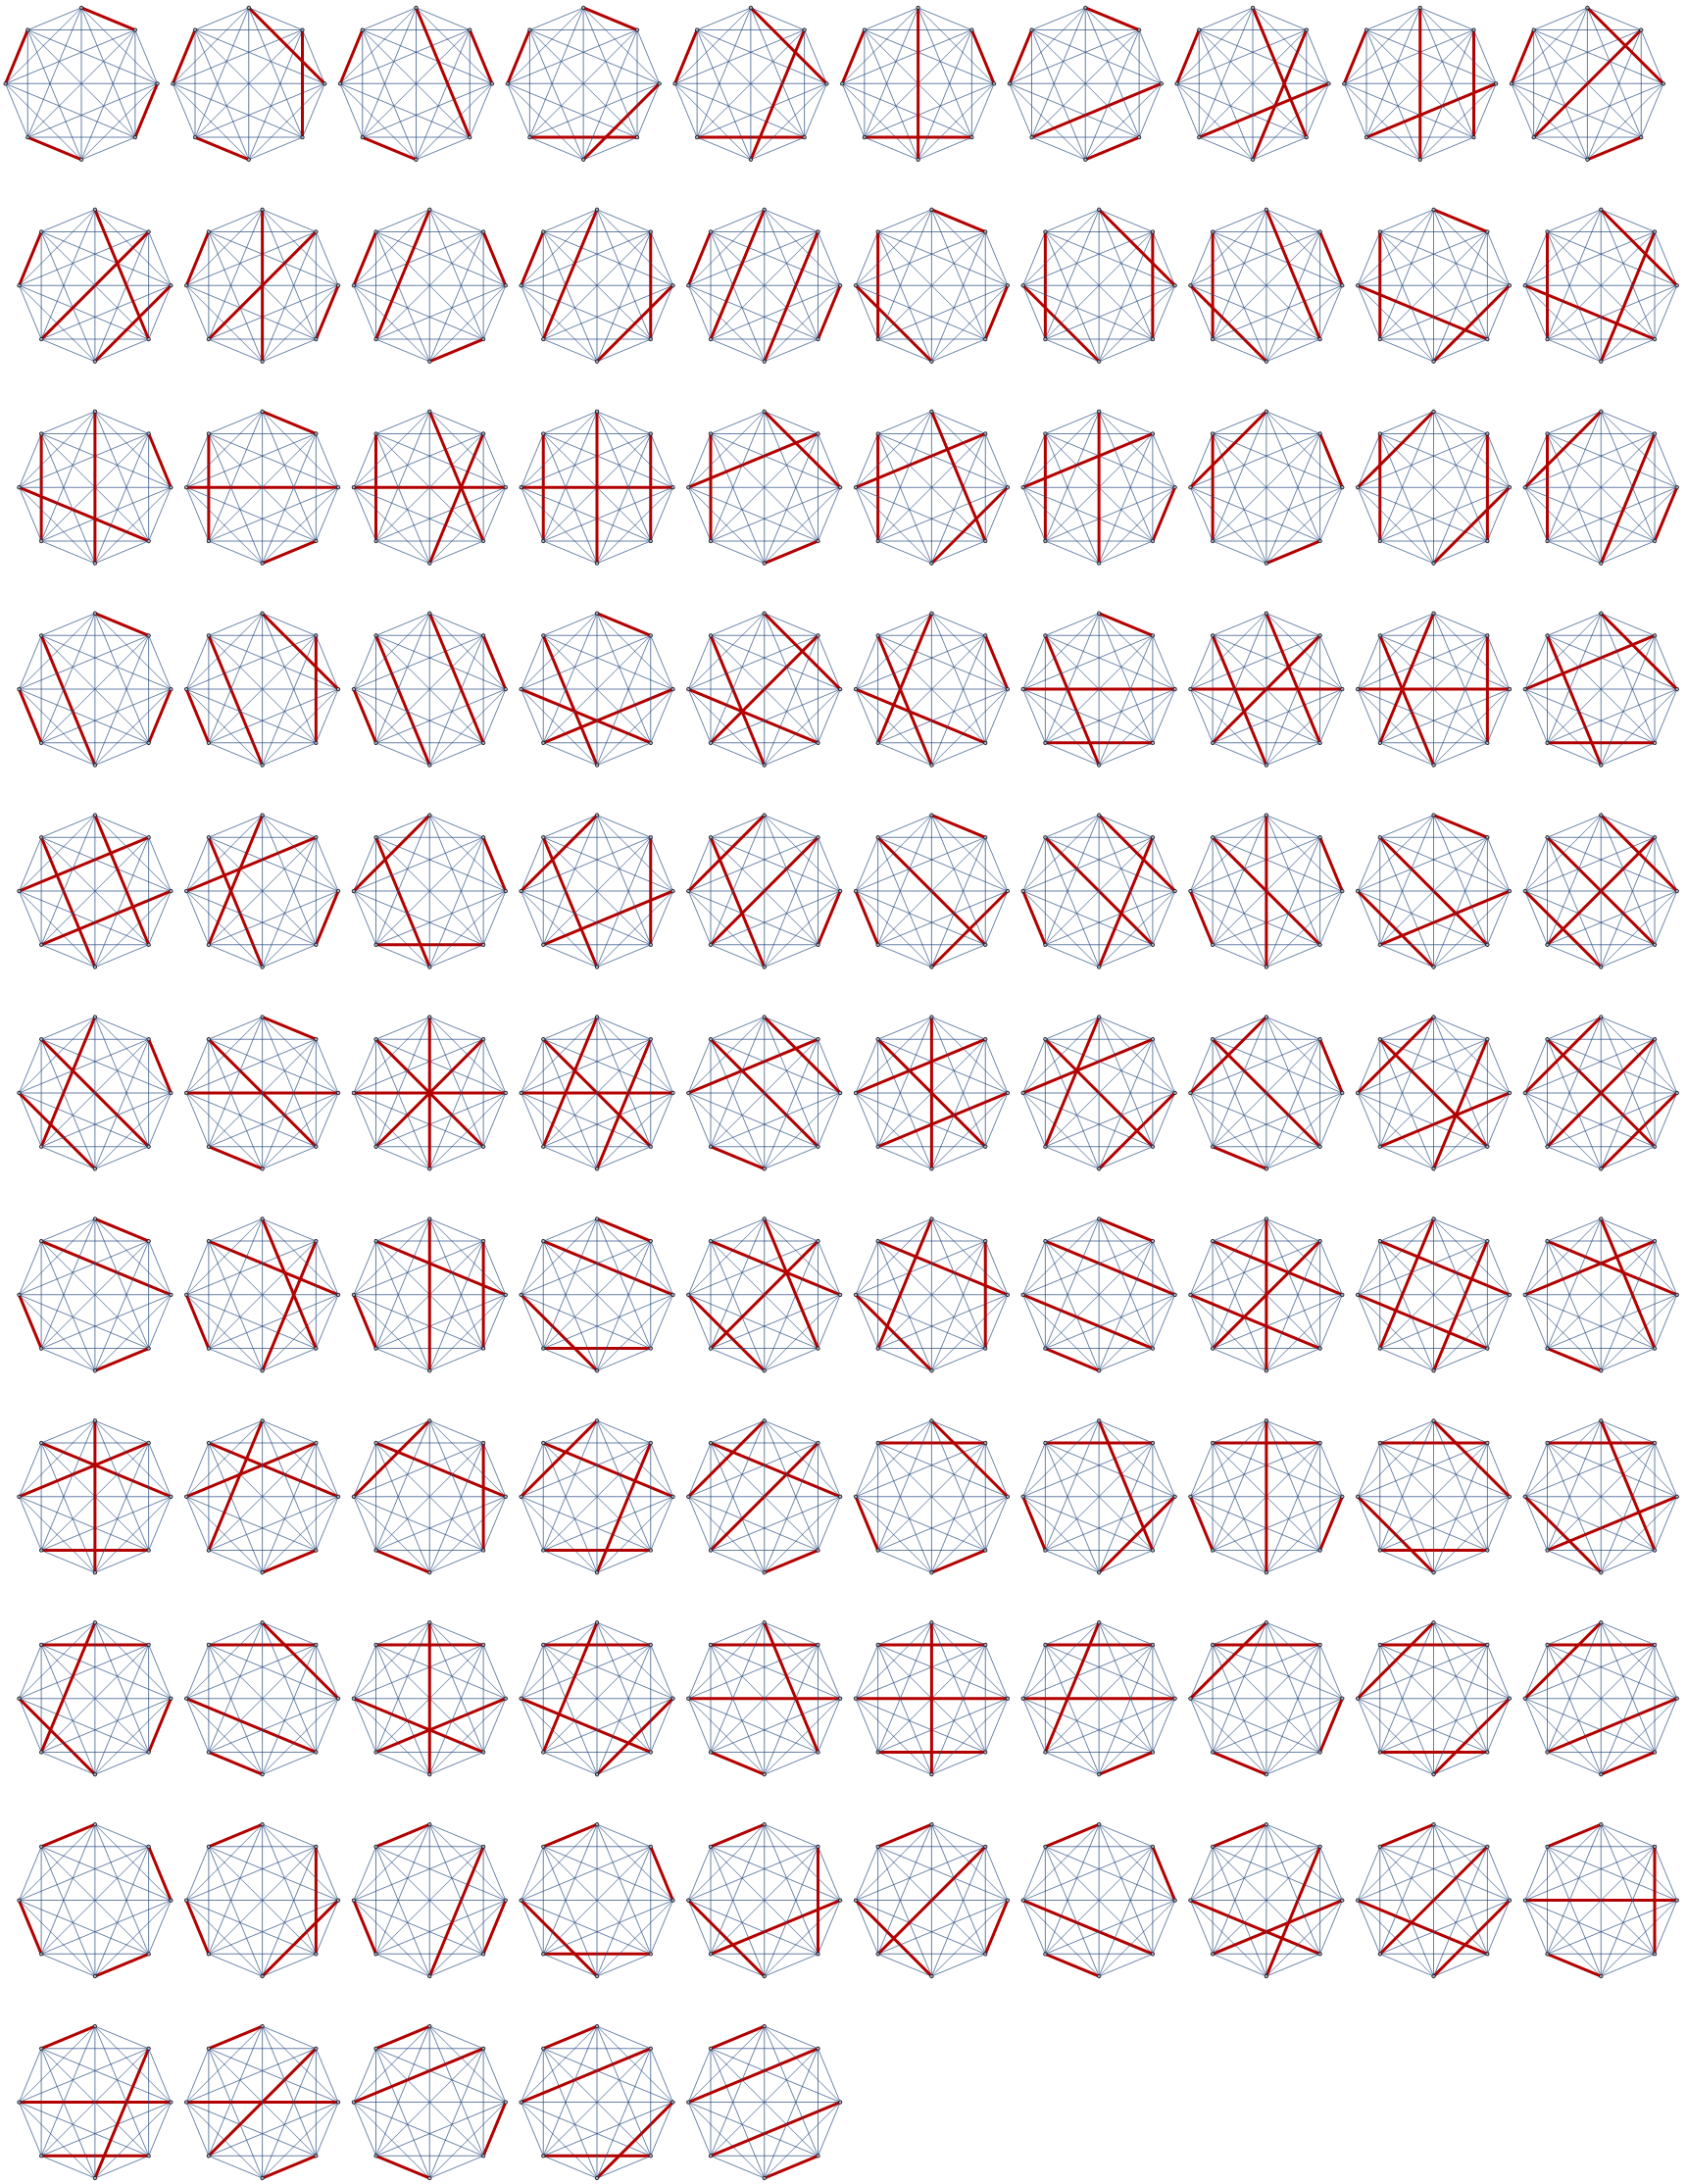
\includegraphics[width=11cm]{Images/newk8perfectmatching.png}
    \caption{$(2\cdot4-1)!!=7!!=105$ perfect matchings of $K_{8}$}
    \label{fig:k8matching}
\end{figure}
\clearpage

\begin{figure}[!htb]
    \centering
    \begin{tabular}{|l|l|l|l|l|l|}
    \hline
        11223344 & 12442133 & 22144133 & 33221441 & 11223443 & 12442331 \\ \hline
        22144331 & 33224411 & 11224433 & 12443321 & 22331144 & 33244211 \\ \hline
        11233244 & 13312244 & 22331441 & 33441122 & 11233442 & 13312442 \\ \hline
        22334411 & 33441221 & 11234432 & 13314422 & 22344311 & 33442211 \\ \hline
        11244233 & 13322144 & 22441133 & 34431122 & 11244332 & 13322441 \\ \hline
        22441331 & 34431221 & 11332244 & 13324421 & 22443311 & 34432211 \\ \hline
        11332442 & 13344122 & 23321144 & 44112233 & 11334422 & 13344221 \\ \hline
        23321441 & 44112332 & 11344322 & 13443122 & 23324411 & 44113322 \\ \hline
        11442233 & 13443221 & 23344211 & 44122133 & 11442332 & 14412233 \\ \hline
        23443211 & 44122331 & 11443322 & 14412332 & 24421133 & 44123321 \\ \hline
        12213344 & 14413322 & 24421331 & 44133122 & 12213443 & 14422133 \\ \hline
        24423311 & 44133221 & 12214433 & 14422331 & 24433211 & 44221133 \\ \hline
        12233144 & 14423321 & 33112244 & 44221331 & 12233441 & 14433122 \\ \hline
        33112442 & 44223311 & 12234431 & 14433221 & 33114422 & 44233211 \\ \hline
        12244133 & 22113344 & 33122144 & 44331122 & 12244331 & 22113443 \\ \hline
        33122441 & 44331221 & 12332144 & 22114433 & 33124421 & 44332211 \\ \hline
        12332441 & 22133144 & 33144122 & 12334421 & 22133441 & 33144221 \\ \hline
        12344321 & 22134431 & 33221144 &  &  &  \\ \hline
    \end{tabular}
    \caption{$7!!=105$ Stirling permutations of order 4}
    \label{fig:stirling4}
\end{figure}\par
The Stirling permutations for any given $n$ can be constructed by following an Euler path on an ordered tree with $n$ edges. Examples of the constructions of order 3 and 4 is shown below.\cite{stackstirling}
\begin{figure}[!htb]
    \centering
    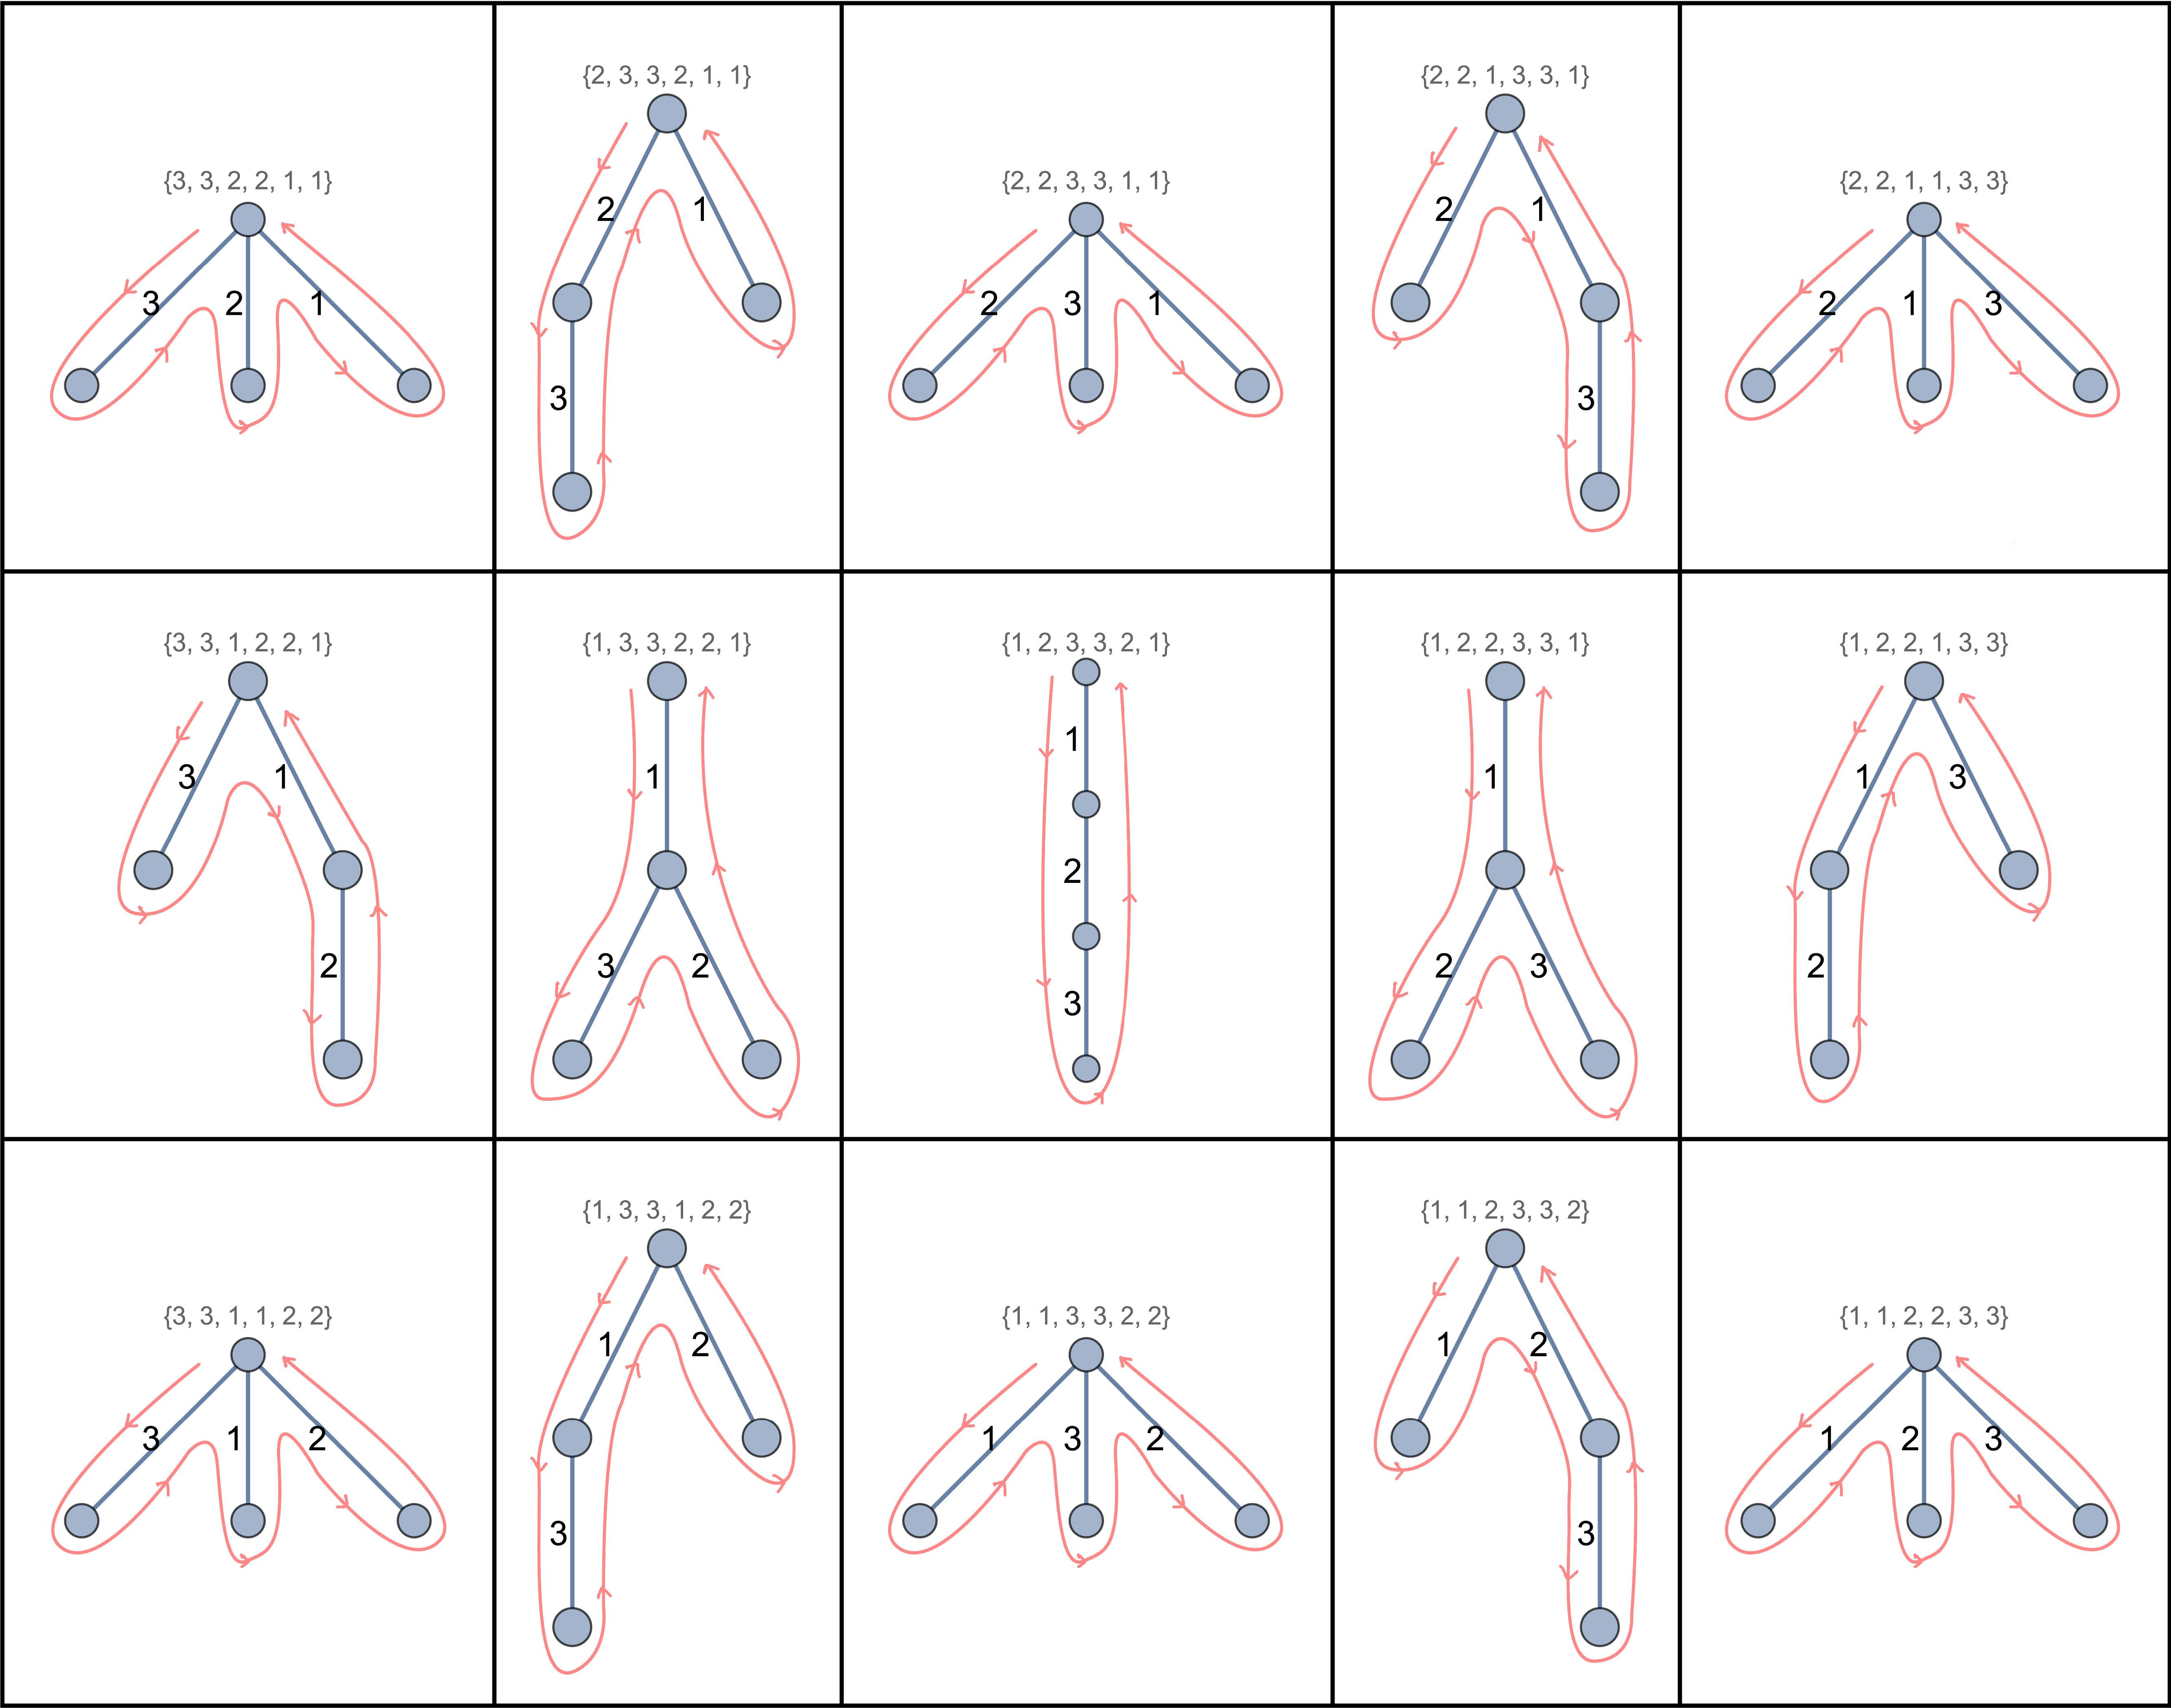
\includegraphics[width=10cm]{Images/smalleulertours.jpg}
    \caption{Construction of Stirling permutations of order 3}
    \label{fig:stirling3graph}
\end{figure}
\clearpage
\begin{figure}[!htb]
    \centering
    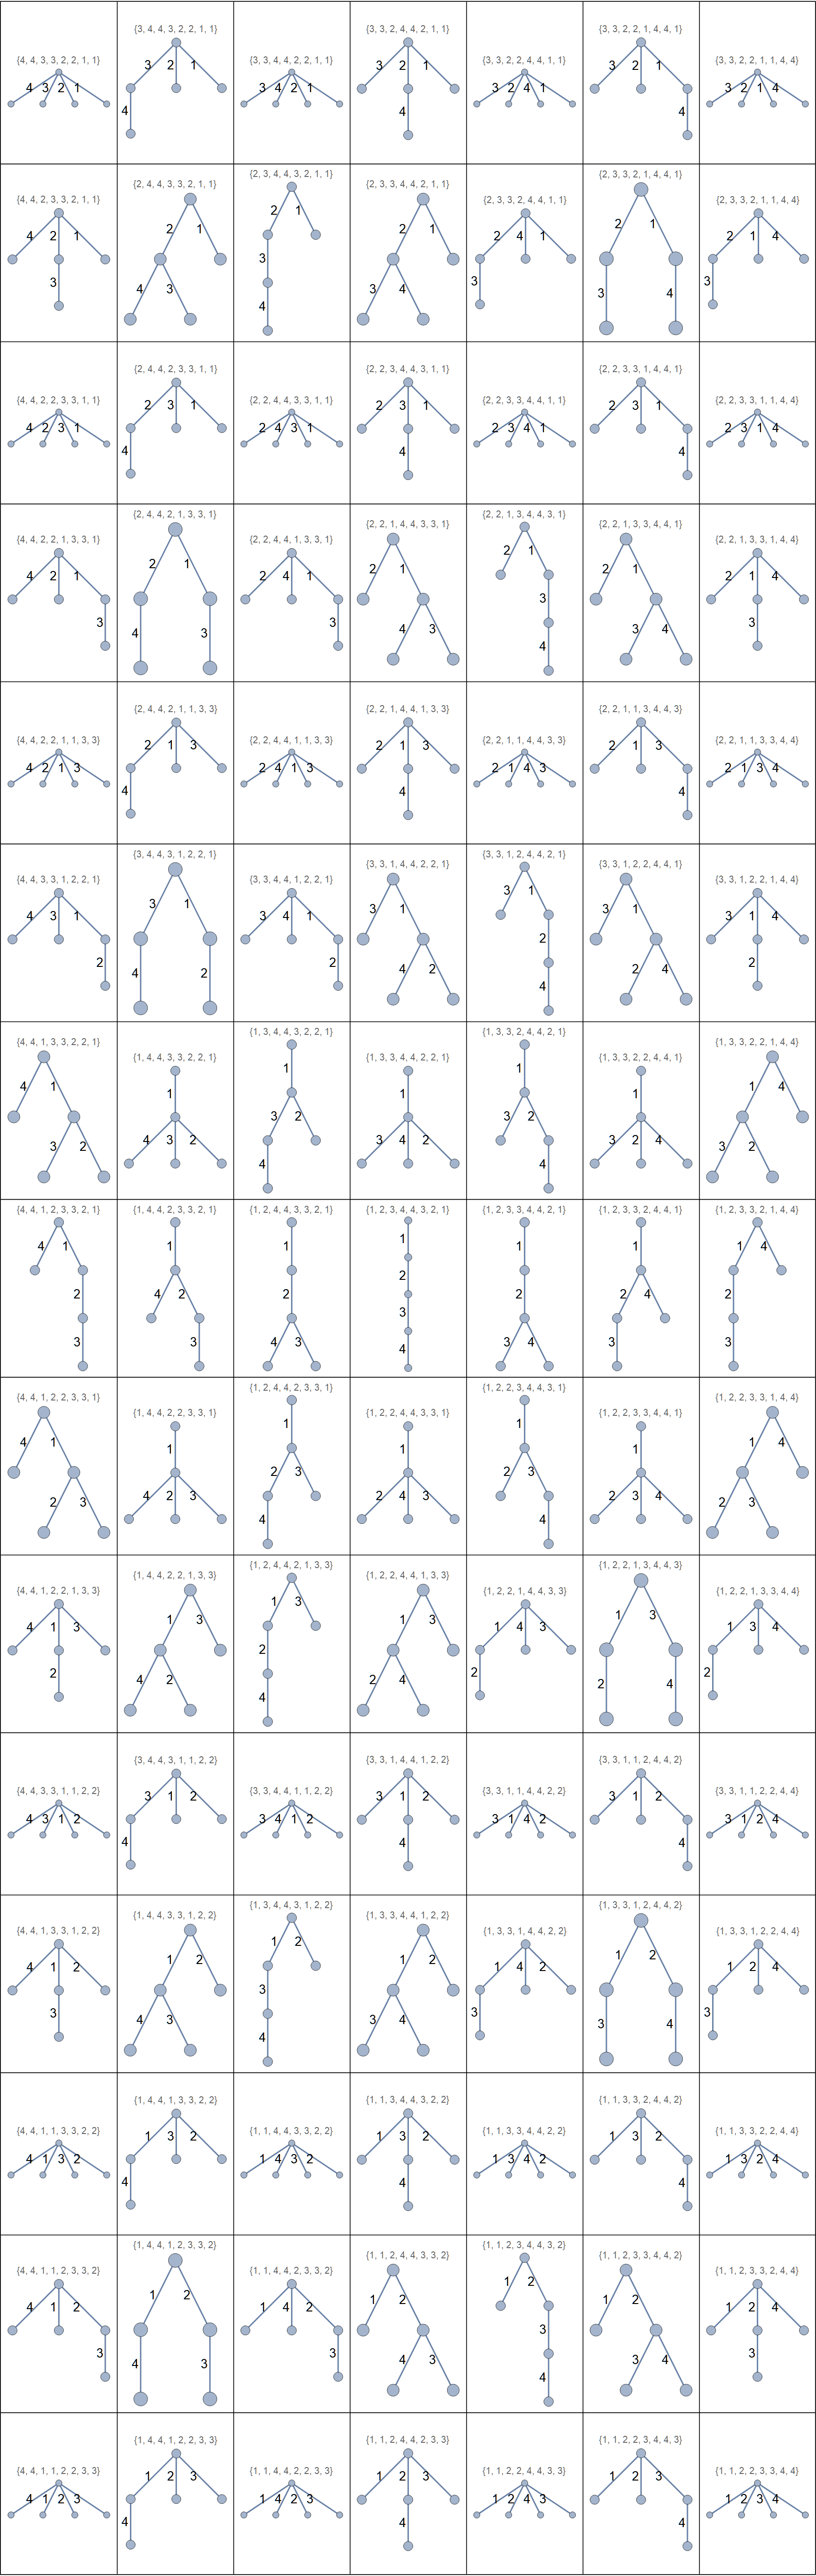
\includegraphics[height=\textheight]{Images/neweulertours.png}
    \caption{Construction of Stirling permutations of order 4}
    \label{fig:stirling4graph}
\end{figure}
\clearpage
%------------------------------------------------

\subsection{Definition of Multifactorial}
We shall now formally define the multifactorial. The simplest way to understand the multifactorial is by comparing it with the factorial. We know that the factorial is defined as follows:
\begin{align*}
    n!&=n\cdot(n-1)\cdot(n-2)\cdot(n-3)\dots && \textit{Terminates with 1}
    \intertext{Using steps of larger integer values we get,}
    n!! &=n\cdot(n-2)\cdot(n-4)\cdot(n-6)\dots && \textit{Terminates with 2 or 1}\\
    n!!! &=n\cdot(n-3)\cdot(n-6)\cdot(n-9)\dots && \textit{Terminates with 3, 2 or 1}\\
    & \vdots
\end{align*}\par
Using this we can alternatively define the multifactorial of any $n>0$ of order $k>0$ as the follows:
\begin{align}
    n!_{(k)}&=\prod_{j=0}^{q}kj+r && \text{where}\ n=kq+r,q\geq 0, \text{and}\ 1\leq r \leq k\\
    &=1 && n=0 \nonumber
\end{align}\par
The above definition is identical to the recursive relation:
\begin{align}
    n!_{(k)} =   \begin{cases}
1 & \text{if $n=0$} \\
n & \text{if $0<n\leq k$} \\   n\left((n-k)!_{(k)}\right) & \text{if $n>k$}   \end{cases}
\end{align}

%----------------------------------------------------------------------------------------
%	Section 3
%----------------------------------------------------------------------------------------

\section{Reciprocal Multifactorial Series}

Now that we have defined multifactorials we can define the Reciprocal Multifactorial Series.
\subsection{Definition}
The Reciprocal Multifactorial Series for multifactorial of order $k$ is defined as the follows:
\begin{align}
    m(k)&=\sum_{n=0}^{\infty}\frac{1}{n!_{(k)}}=1+\sum_{r=1}^{k}\sum_{q=0}^{\infty}\frac{1}{(kq+r)\underbrace{!\dots!}_{\text{k times}}}
\end{align}\par
\emph{(The 1 in the above representation is due to $0!_{(k)=1.)}$.} We all know of the convergence for the famous case of m(1) which equates to $e$. However in general we can test the convergence of m(k) individually using the ratio test.
\clearpage
\textbf{Example 1: Testing Convergence of m(1)}
\begin{align*}
    S_n=\sum_{n=0}^{\infty}\frac{1}{n!}
\end{align*}
\begin{align*}
    L=\lim_{n\rightarrow \infty}\left | \frac{a_{n+1}}{a_{n}} \right|&=\lim_{n\rightarrow \infty} \left |\frac{\frac{1}{(n+1)!}}{\frac{1}{n!}}\right|\\
    &=\lim_{n\rightarrow \infty}\frac{n!}{(n+1)!}\\
    &=\lim_{n\rightarrow \infty}\frac{1}{n+1}=0
\end{align*}
\text{\;\;\;\;\;\;\; Since $L<1$, by Ratio Test we can say that $S_n$ is absolutely convergent. \hfill $\square$} 
\vfill 
\textbf{Example 2: Testing Convergence of m(2)}
\begin{align*}
    S_n &=\sum_{n=0}^{\infty}\frac{1}{n!!}\\
    \text{Consider the relations}\ &\text{between}\ n!\ \text{and}\ n!!.\\
    2n!! &= 2^n n! && \text{where n is even}\\
    (2n-1)!! &= \frac{(2n+1)!}{2^n n!} && \text{where n is odd}
\end{align*}
\text{\;\;\;\;\;\;\;Case I: $n$ is even, $n+1$ is odd}
\begin{align*}
    L=\lim_{n\rightarrow \infty}\left | \frac{a_{n+1}}{a_{n}} \right|&=\lim_{n\rightarrow \infty}\left | \frac{\frac{1}{\frac{(2(n+1))!}{2^{n+1}(n+1)!}}}{\frac{1}{2^n n!}} \right |\\
    &=\lim_{n\rightarrow \infty}\frac{2^n n!}{\frac{(2 (n+1))!}{2^{n+1} (n+1)!}}=0
\end{align*}
\text{\;\;\;\;\;\;\;Case II: $n$ is odd, $n+1$ is even}
\begin{align*}
    L=\lim_{n\rightarrow \infty}\left | \frac{a_{n+1}}{a_{n}} \right|&=\lim_{n\rightarrow \infty}\left | \frac{\frac{1}{2^{n+1}(n+1)!}}{\frac{1}{\frac{(2n)!}{2^n n!}}} \right |\\
    &=\lim_{n\rightarrow \infty}\frac{\frac{(2n)!}{2^n n!}}{2^{n+1}(n+1)!}=0
\end{align*}
\text{\;\;\;\;\;\;\;Since in both cases $L<1$, by Ratio test we can say that $S_n$ is}\\ 
absolutely convergent. \hfill $\square$

\par
The above used relations between the double factorial and factorial can be derived in the following manner.
\begin{align*}
    (2n)!!&=(2n)(2n-2)(2n-4) \cdots 2\\
    &=[2(n)][2(n-1)][2(n-2)] \cdots 2\\
    &= 2^n n! \QED \\
    (2n+1)!!2^n n! &=[(2n+1)(2n-1)\cdots 1][2n][2(n-1)][2(n-2)]\cdots2\\
    &=[(2n+1)(2n-1) \cdots 1] [2n(2n-2)(2n-4) \cdots 2]\\
    &=(2n+1)(2n)(2n-1)(2n-2)\cdots 2\\
    &=(2n+1)!
    \QED
\end{align*}
\par To read about some more proprieties of the double factorial in detail refer to "Double Factorial"- MathWorld.\cite{doublefactorial}
\subsection{Computations of Reciprocal Multifactorial Series}
We can examine the convergence of a few terms of m(k) computationally. The below table enumerates m(1) through to m(10) summed up from n=0 to n=150 and rounded to 10 significant digits. These are the first ten Reciprocal Multifactorial Constants (RMFCs).

\begin{table}[h!]
\centering
\begin{tabular}{@{}cc@{}}
\toprule
m(k) & $\sum_{n=0}^{2000}\frac{1}{n!_{(k)}}$  \\ & Rounded to 10 significant digits \\ \midrule
m(1) & 2.718281828 \\
m(2) & 3.059407405 \\
m(3) & 3.298913538 \\
m(4) & 3.485944977 \\
m(5) & 3.640224468 \\
m(6) & 3.771902396 \\
m(7) & 3.886959654 \\
m(8) & 3.989241213 \\
m(9) & 4.081375520 \\
m(10) & 4.165243766 \\ \bottomrule
\end{tabular}
\caption{ Computed values of first 10 RMFCs}
\label{tab:summationvalues}
\end{table}\par
The values can be seen on the OEIS \cite{oeis}. Below we have displayed the first 50 partial sums of first 10 Reciprocal Multifactorial Series. The upward trend of the convergence can be easily seen in these plots.
\begin{figure}[!hbp]
    \centering
    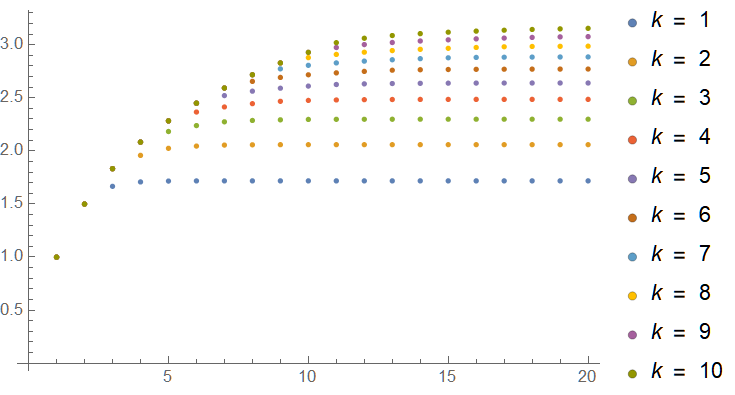
\includegraphics[width=13cm]{Images/20partialsums.png}
    \caption{First 20 partial sums of first 10 Reciprocal Multifactorial Series}
    \label{fig:20partialsums}
\end{figure}
\begin{figure}[!htp]
    \centering
    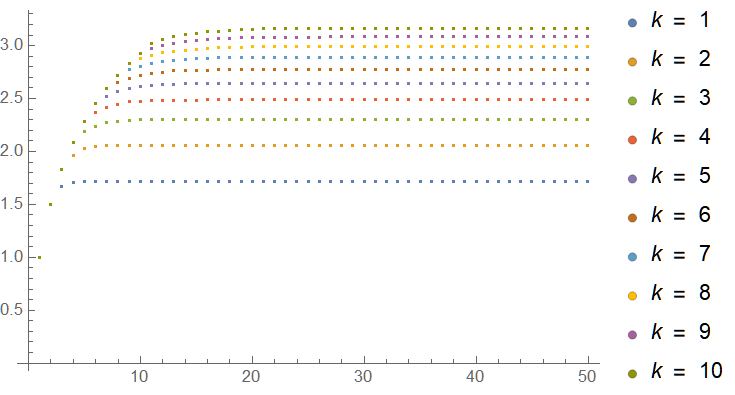
\includegraphics[width=13cm]{Images/Plotofm1tom10.png}
    \caption{First 50 partial sums of first 10 Reciprocal Multifactorial Series}
    \label{fig:50partialsums}
\end{figure}
\clearpage

%----------------------------------------------------------------------------------------
%	Section 4
%----------------------------------------------------------------------------------------

\section{Closed form formula for RMFCs}
In this section we shall prove the closed form formula for the $k^{th}$ reciprocal multifactorial constant.
\subsection{Prerequisite definitions}
We shall first state a few important definitions needed for the proof. \cite{gamma} \cite{beta} \cite{incompletegamma}
\begin{align}
    &\text{Gamma Function } \Gamma (z)=\int_0^{\infty}x^{z-1}e^{-x}dx\text{ for } \text{Re}(z)>0
    \numberwithin{equation}{subsection}\\
    &\text{Beta Function }  \text{B}(x, y)=\int_0^1 t^{x-1}(1-t)^{y-1} dt \text{ for } \text{Re}(x), \text{Re}(y)>0 \\
    &\text{B}(x,y)=\frac{\Gamma(x)\Gamma(y)}{\Gamma(x+y)}\\
    &\text{Lower incomplete gamma function } \gamma (a, x) = \int_0^x t^{a-1} e^{-t} dt
\end{align}
\subsection{Proof for closed form formula for RMFCs}
Let us begin by proving a lemma that is needed for the final theorem.
\numberwithin{equation}{section}
\begin{lemma}
Relation between $k^{th}$ multifactorial and Beta function.
\end{lemma}
\textbf{Proof: }Recall the definition of multifactorial as described in Eq. 2.1.
\begin{align*}
    n\underbrace{!\ldots!}_{\text{k times}}=n!_{(k)}=\prod_{j=0}^q(kj+r)&=k^{q+1}\prod_{j=0}^q\left(j+\frac rk\right)\\
&=k^{q+1}\frac{\Gamma(q+1+\frac{r}{k})}{\Gamma(r/k)}\\
&=\frac{k^{q+1}\Gamma(q+1)}{\mathrm{B}\left (\dfrac{r}{k}, q+1\right )} && \text{(using 4.1.3)}\\
&=\frac{k^{q+1}q!}{\mathrm{B}\left (\dfrac{r}{k}, q+1\right )} && \text{(q is a positive integer)}
\end{align*}
We now have a relation between the multifactorial and the Beta function given as follows.
\begin{align}
    n!_{(k)}=\frac{k^{q+1}q!}{\mathrm{B}\left (\dfrac{r}{k}, q+1\right )}
\end{align}
Therefore, we have 
\begin{align*}
    \frac{1}{n!_{(k)}}=\frac{\mathrm{B}\left (\dfrac{r}{k}, q+1\right )}{k^{q+1}q!} \QED
\end{align*}\par
We have now established all definitions we need to prove the closed form formula for RMFCs. The proof involves using the Beta function representation of the multifactorial and then proceeding to simplify the function to arrive at a closed form formula.\cite{RMFCwolfram}\cite{stackproof}
\begin{theorem}A closed form formula for Reciprocal Multifactorial Constants is given by the following expression
$$m(k)=1+\frac{e^{1/k}}{k}\sum_{r=1}^{k}k^{r/k}\gamma\left ( \frac{r}{k}, \frac{1}{k} \right )$$
\end{theorem}\par 
\textbf{Proof: }Recall definition 3.1 for reciprocal multifactorial series.
\begin{align*}
    m(k)&=\sum_{n=0}^{\infty}\frac{1}{n!_{(k)}}=1+\sum_{r=1}^{k}\sum_{q=0}^{\infty}\frac{1}{(kq+r)\underbrace{!\dots!}_{\text{k times}}}\\
    \intertext{Now, using Lemma 4.1 we get,}
    &=1+\sum_{r=1}^k\sum_{q=0}^\infty\frac{1}{k^{q+1}q!}\mathrm{B}\left(\frac rk,q+1\right)
    \intertext{Using the integral definition for the Beta function (see 4.1.2) we can say,}
    &=1+\sum_{r=1}^k\sum_{q=0}^\infty\frac{1}{k^{q+1}q!}\int_0^1 t^{r/k-1}(1-t)^q\,dt\\
    &=1+\sum_{r=1}^k\sum_{q=0}^\infty\frac{1}{k k^{q}q!}\int_0^1 t^{r/k-1}(1-t)^q\,dt
    \intertext{We can now re-arrange the integral and summation signs (this is possible since the expression is strictly greater than 0)..}
    &=1+\frac1k\sum_{r=1}^k\int_0^1 t^{r/k-1}\sum_{q=0}^\infty\frac1{q!}\left(\frac{1-t}{k}\right)^q dt
    \intertext{Since $\sum_{n=0}^{\infty}\frac{x^n}{n!}=e^x$ we have,}
    &=1+\frac1k\sum_{r=1}^k\int_0^1 t^{r/k-1}e^{(1-t)/k}\,dt
    \intertext{Taking $t=kx$ we simplify the function as follows,}
    &=1+\frac1k\sum_{r=1}^k\int_0^{1/k} (kx)^{r/k-1}e^{(1-kx)/k}\,k dx\\
    &=1+\frac{1}{k}\sum_{r=1}^k\int_0^{1/k} k^{r/k-1}x^{r/k-1}e^{1/k}e^{-x}\,k dx\\
    &=1+\frac{e^{1/k}}{k}\sum_{r=1}^k\int_0^{1/k} k^{r/k}x^{r/k-1}e^{-x}\, dx
    \\&=1+\frac{e^{1/k}}k\sum_{r=1}^k k^{r/k}\int_0^{1/k}x^{r/k-1}e^{-x}\,dx
    \intertext{Finally using the definition for incomplete gamma function (see 4.1.4),}
    &=1+\frac{e^{1/k}}k\sum_{r=1}^k k^{r/k}\gamma \left (\frac{r}{k}, \frac{1}{k} \right) 
    \QED
\end{align*}
\clearpage
\subsection{Computation of RMFCs using the closed form formula}
\par
Using the closed form formula allows us to compute RMFCs with greater computational efficiency. Below we have listed the first ten RMFCs calculated up to 20 decimal place accuracy.
\begin{table}[h!]
\centering
\begin{tabular}{cc}
\hline
m(k) & Computed RMFCs \\ \hline
m(1) & 2.7182818284590452354 \\
m(2) & 3.0594074053425761445 \\
m(3) & 3.2989135380884190034 \\
m(4) & 3.4859449774535577452 \\
m(5) & 3.6402244677338097342 \\
m(6) & 3.7719023962117584357 \\
m(7) & 3.8869596537408434954 \\
m(8) & 3.9892412126901365441 \\
m(9) & 4.0813755201688985441 \\
m(10) & 4.1652437655583845908 \\ \hline
\end{tabular}
\caption{ Computed values of first 10 RMFCs using closed form formula (20 digit accuracy)}
\label{tab:closedformrmfcvalues}
\end{table}
\par We can further analyze the time taken for the computer to execute both the series definition and the closed form formula definition of a RMFCs.\par
We shall first test the two functions in their ability to calculate larger order RMFCs for an arbitrary decimal accuracy.\par
The below plots displays the time taken for the computer to compute a list of the first k RMFCs (k ranging from 1 to 200) up to a 50 digit accuracy. Using the series definition (in red) and the closed form definition (in blue).\par
We can see from the below plots that computing higher order RMFCs using the series definition is slightly slower to in comparison with the closed form formula.
\begin{figure}[!hbp]
    \centering
    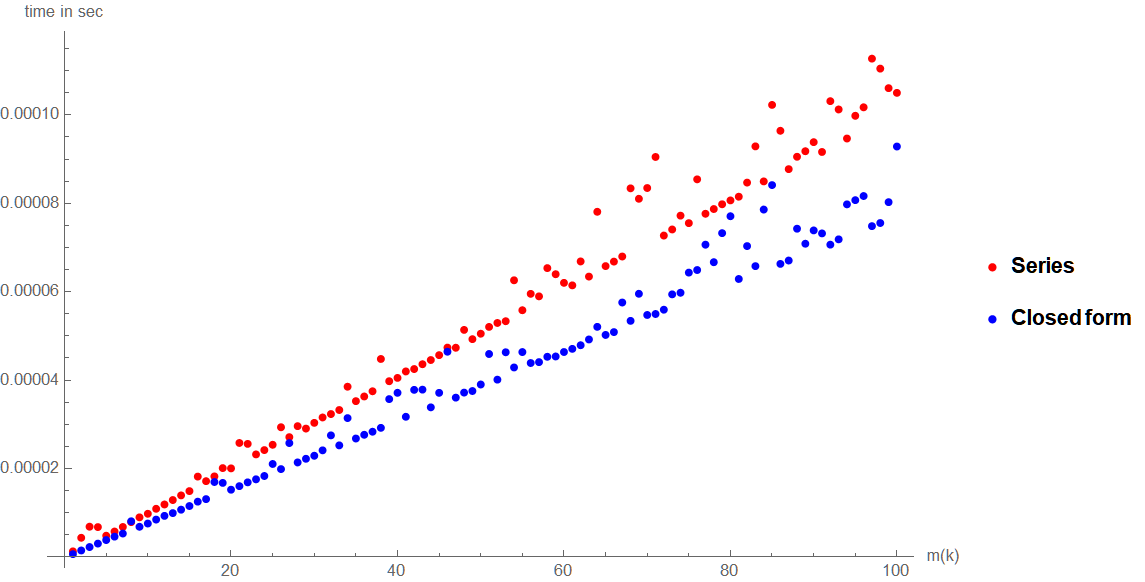
\includegraphics[width=13cm]{Images/first100RMFCseriesvsclosedform.png}
    \caption{Time taken to compute a list of first k RMFCs (k ranging from 1 to 100) up to 50 digit accuracy.}
    \label{fig:timecompfirst100rmfcs}
\end{figure}\\
\begin{figure}[!hbp]
    \centering
    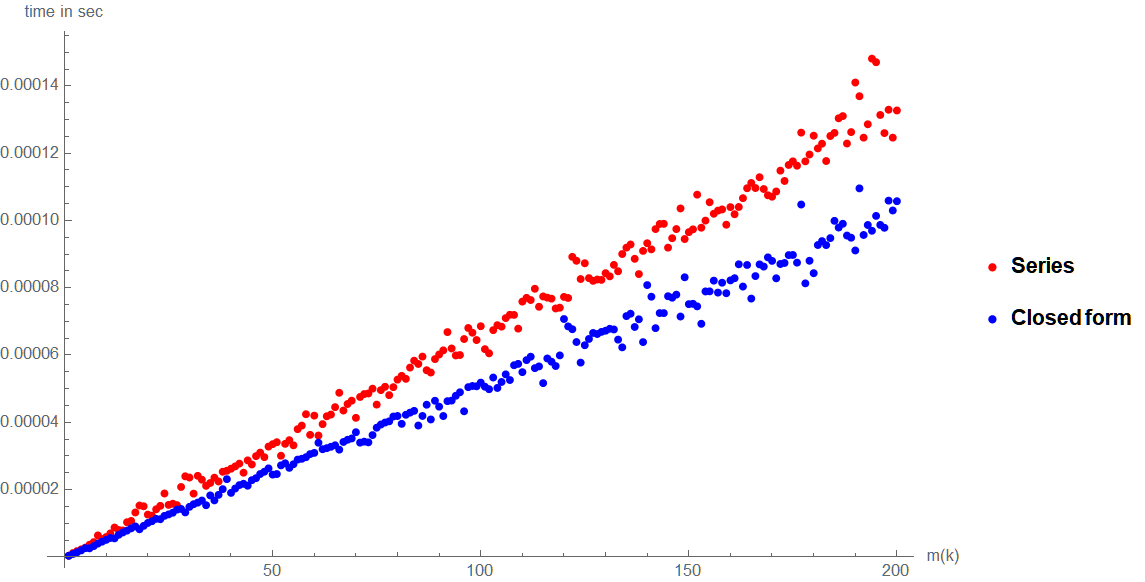
\includegraphics[width=13cm]{Images/first200RMFCseriesvsclosedform.png}
    \caption{Time taken to compute a list of first k RMFCs (k ranging from 1 to 200) up to 50 digit accuracy.}
    \label{fig:timecompfirst200rmfcs}
\end{figure}
\clearpage
We will now take a look at the individual computations of some arbitrary RMFCs for increasing order of digit accuracy.\par
The below plots display the comparison between two functions for simultaneous computation of the first 10 RMFCs with higher levels of digit accuracy.
\begin{figure}[!hbp]
    \centering
    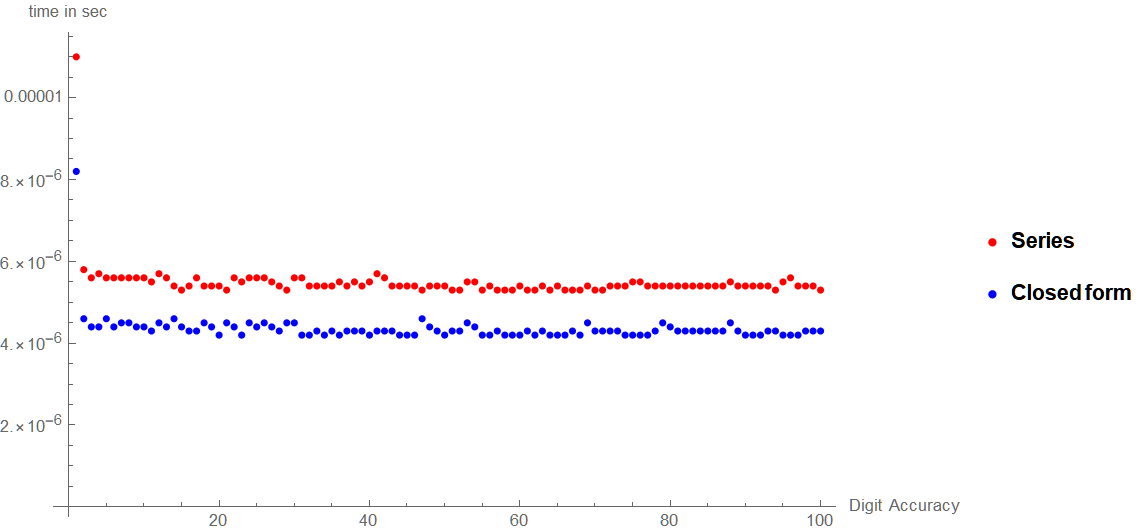
\includegraphics[width=13cm]{Images/first100digitsaccuracy.png}
    \caption{Time taken to compute first 10 RMFCs with increasing accuracy up to 100 digit accuracy.}
    \label{fig:timecomp10rmfc100digit}
\end{figure}
\begin{figure}[!hbp]
    \centering
    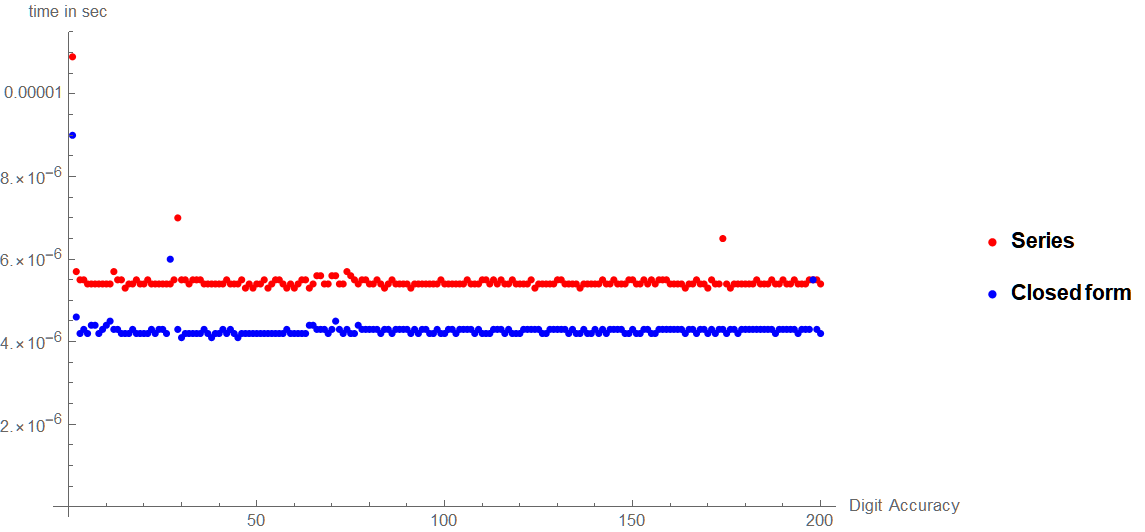
\includegraphics[width=13cm]{Images/first200digitsaccuracy.png}
    \caption{Time taken to compute first 10 RMFCs with increasing accuracy up to 200 digit accuracy.}
    \label{fig:timecomp10rmfc200digit}
\end{figure}\par
From the above two plots it is seen that the closed form formula is computationally faster than the series definition for obtaining more accurate values of RMFCs. 

%----------------------------------------------------------------------------------------
%	Section 5
%----------------------------------------------------------------------------------------

\section{Asymptotics of Reciprocal Multifactorial Series}
\par In this section we will examine the asymptotic behaviour of the RMFCs, i.e. we will examine what happens to the RMFC, m(k), as k approaches positive infinity.
\par A keen reader might have noticed that the computed values of RMFCs displayed in Tables 1 and 2 all seem to be increasing for higher orders.
\par This can be observed from the below graph.
\begin{figure}[!hbp]
    \centering
    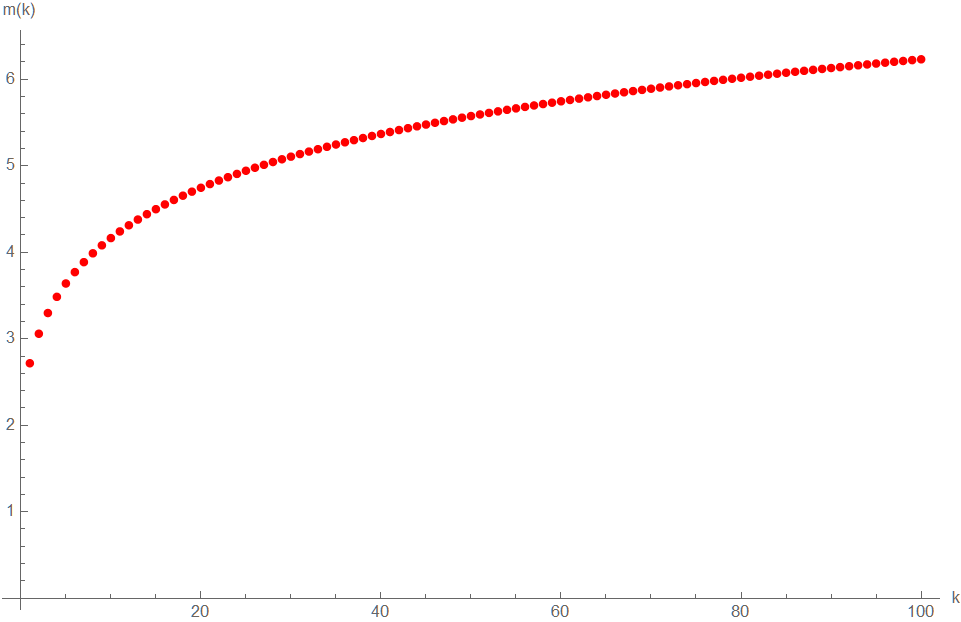
\includegraphics[width=10cm]{Images/first100RMFCs.png}
    \caption{First 100 RMFCs}
    \label{fig:first100rmfcs}
\end{figure}
\subsection{Casual observation}
\par We shall first motivate the concept that RMFCs get arbitrarily larger by a simple observation based on definition for a multifactorial. Recall Definition 2.2,
\begin{align*}
    n!_{(k)} =   \begin{cases}
1 & \text{if $n=0$} \\
n & \text{if $0<n\leq k$} \\   n\left((n-k)!_{(k)}\right) & \text{if $n>k$}   \end{cases}
\end{align*}\par
Observe carefully the second line that says $n!_{(k)}=n,\ \text{if } 0<n\leq k.$
One can tell that as $k$ approaches infinity every $q!_{(k)}$ for $q<k$ will simply be equal to $q$. As such the Reciprocal Multifactorial Series will simply resemble $$1+\sum_{i=1}^k \frac{1}{i}=1+H_k \text{, as k approaches infinity.}$$
\par Where $H_k$ is the $k^{th}$ harmonic number. We shall show this more rigorously in the following sections.
\subsection{Proof of divergence}
We will begin with a result achieved in the proof of the closed form formula (line 6 of the proof) and proceed to prove the assertion made in the previous section.\cite{stackasymptote}
\numberwithin{corollary}{section}
\begin{theorem}
$\lim_{k\rightarrow \infty} m(k) = 1+H_k$
\end{theorem}
\textbf{Proof: }Consider the following expression (shown in Theorem 4.2)
\begin{align*}
    m(k)&=1+\frac1k\sum_{r=1}^k\int_0^1 t^{r/k-1}e^{(1-t)/k}\,dt\\
    &=1+\frac{e^{1/k}}{k}\sum_{r=1}^k\int_0^1 t^{r/k-1}e^{-t/k}\,dt
    \intertext{Observe that $e^{-t/k}=1-(1-e^{-t/k})$}
    &=1+\frac{e^{1/k}}{k}\sum_{r=1}^k\int_0^1 t^{r/k-1}(1-(1-e^{-t/k}))\,dt
    \intertext{Since, $\int_0^1 t^{r/k-1}\,dt=\frac{k}{r}$, we can further simplify the above expression as}
    &=1+\frac{e^{1/k}}{k}\sum_{r=1}^k \left( \frac{k}{r}-\int_0^1 t^{r/k-1}(1-e^{-t/k})\,dt \right)\\
    &=1+e^{1/k} \left(H_k-\frac{1}{k} \int_0^1 \sum_{r=1}^k t^{r/k}\frac{(1-e^{-t/k})}{t}\,dt \right)\\
    &=1+e^{1/k} \left(H_k-\frac1k\int_0^1\frac{(1-t)(1-e^{-t/k})}{t(t^{-1/k}-1)}\,dt.\right)
    \intertext{Replacing $\frac1k\int_0^1\frac{(1-t)(1-e^{-t/k})}{t(t^{-1/k}-1)}\,dt.$ with $\Delta k$ we get, }
    m(k)&=1+e^{1/k}\left( H_k - \Delta k \right)
    \intertext{Taking the limit as k approaches infinity we get,}
    \lim_{k\rightarrow \infty} m(k)&=\lim_{k\rightarrow \infty} 1+e^{1/k}(H_k - \Delta k)\\
    \lim_{k\rightarrow \infty} m(k)&=1+H_k \QED
\end{align*}
\subsection{Alternate proof of divergence}
In this section we will provide an alternate proof for Theorem 5.1. To begin we will prove the a few results about the lower incomplete gamma function.\cite{powerseriesgamma}\par
In this section the notation $x^{(n)}$ will refer to rising factorials, which is defined as $x^{(n)}=x(x+1)(x+2)\dots(x+n-1).$ \cite{risingfactorial}  
\begin{lemma}The power series for the lower incomplete gamma function is
$${\displaystyle \gamma (a,x)=x^{a}e^{-x}\sum _{k=0}^{\infty }{\dfrac {x^{k}}{a^{(k+1)}}}}$$
\end{lemma}
\textbf{Proof: } We will derive the power series by repeated integration by parts. Recall definition (4.1.4)
\begin{align*}
    \gamma (a, x) &= \int_0^x t^{a-1}e^{-t}\ dt
    \intertext{Integrating by parts, $u=e^{-t}, du=-e^{-t} dt, dv=t^{a-1}\ dt, v=\frac{t^a}{a}$}
    &= e^{-x} \cdot \frac{x^a}{a}-\int_0^x \frac{t^a}{a} \cdot (-e^{-t}) dt\\
    &= \frac{e^{-x}x^a}{a}+\frac{1}{a}\int_0^x t^a e^{-t}\ dt\\
    \gamma (a,x)&=\frac{e^{-x}x^a}{a}+\frac{1}{a}\gamma(a+1, x)
    \intertext{This is the recurrence relation, further upon repeated integration by parts we get, }
    &= e^{-x}x^{a} \left( \frac{1}{a}+\frac{x}{a(a+1)}+\frac{x^2}{a(a+1)(a+2)}\dots \right)\\
    &= x^{a}e^{-x}\sum_{k=0}^\infty\frac{x^k}{a^{(k+1)}} \QED
\end{align*}
Now we will prove another useful lemma regarding the limit of the lower incomplete gamma function.
\clearpage
\begin{lemma}
$$ {\frac {\gamma (a,x)}{x^{a}}}\rightarrow {\frac {1}{a}}, \textup{ as, } x \rightarrow 0$$
\end{lemma}
\textbf{Proof: } We will begin by using the power series for the lower incomplete gamma function.
\begin{align*}
    \gamma(a,x)&=x^{a}e^{-x}\sum_{k=0}^\infty\frac{x^k}{a^{(k+1)}}\\
    \frac {\gamma (a,x)}{x^{a}}&=e^{-x}\left( \frac{1}{a}+\frac{x}{a(a+1)}+\frac{x^2}{a(a+1)(a+2)}\dots \right)
    \intertext{As $x \rightarrow 0, e^{-x} \rightarrow 1$ and all terms with $x$ in the numerator approach 0.}
\end{align*}
\vspace{-1.5cm}
\begin{align*}
    \frac {\gamma (a,x)}{x^{a}}\rightarrow \frac{1}{a} \text{ as, } x\rightarrow 0 \QED
\end{align*}
\begin{theorem}
$$\lim_{k\rightarrow \infty}m(k)=1+H_k$$
\end{theorem}
\textbf{Proof: } Using the result of the closed form formula for RMFCs (Theorem 4.2),
\begin{align*}
    m(k)&=1+\frac{e^{1/k}}k\sum_{r=1}^k k^{r/k}\gamma \left (\frac{r}{k}, \frac{1}{k} \right) 
    \intertext{Taking the limit for $k \rightarrow \infty$ (i.e . $1/k \rightarrow 0$)}
    \lim_{k\rightarrow \infty} m(k) &= 1+ \lim_{k \rightarrow \infty} \frac{e^{1/k}}{k}\sum_{r=1}^k k^{r/k}\gamma 
    \left (\frac{r}{k}, \frac{1}{k} \right)
    \intertext{Using Lemma 5.3 on $\gamma(r/k, 1/k)$ we get}
    \lim_{k\rightarrow \infty} m(k) &= 1+ \lim_{k \rightarrow \infty} \frac{e^{1/k}}{k} \sum_{r=1}^k k^{r/k} 
    \frac{k}{r k^{r/k}}\\
    \lim_{k\rightarrow \infty} m(k) &= 1+ \lim_{k \rightarrow \infty} \frac{e^{1/k}}{k} \sum_{r=1}^k \frac{k}{r}\\
    \lim_{k\rightarrow \infty} m(k) &= 1+ \lim_{k \rightarrow \infty} \frac{e^{1/k}}{k} k H_k\\
    \lim_{k\rightarrow \infty} m(k) &= 1+ \lim_{k \rightarrow \infty} e^{1/k} H_k\\
    \lim_{k\rightarrow \infty} m(k) &= 1+ H_k \QED
\end{align*}
\subsection{Detailed Asymptotics}
\numberwithin{equation}{subsection}
In this section we will mostly refer to the following expression.
\begin{align}
    m(k)=1+e^{1/k}\left( H_k - \Delta k \right)
\end{align}
\par Our goal for the next section is to devise an asymptotic approximation for RMFCs. We will begin by displaying the necessary asymptotic expressions.
\par For $e^{1/k} \text{and} H_k$ we will use known results of its asymptotic expansions are as follows.\cite{expwolfram}\cite{harmonicwolfram}
\begin{align}
    e^{1/k}&=1+\frac{1}{k}+\frac{1}{2 k^2}+O\left (\frac{1}{k^3}\right )\\
    H_k&=\log(k)+\gamma+\frac{1}{2k}-\frac{1}{12k^2}+O\left (\frac{1}{k^4}\right )
\end{align}
\par Where $\gamma$ is the Euler-Mascheroni Constant. \cite{emconstant}
\par We compute the asymptotic expansion of $\Delta k$ using Mathematica. Which results in the following expression.
\begin{align}
    \Delta k=\frac{\log(2)}{k}+\frac{1}{4k^2}\left( -1-\log \frac{9}{4}
    \right) +\frac{1}{48k^3} \left( 5+8 \log \frac{4}{3} \right) + O\left(\frac{1}{k^4} \right)
\end{align}
\subsection{Asymptotic approximations for RMFCs}
\numberwithin{equation}{subsection}
We will use the asymptotic series described above, truncated up to $1^{st}$ and $2^{nd}$ order of $k$ respectively to construct two asymptotic approximations for $m(k)$. Substituting values of (5.4.2), (5.4.3) and (5.4.4) into (5.4.1) we get the following.\\
\textbf{Approximation 1:} Using asymptotic series truncated at $1^{st}$ order terms
\begin{align*}
    m(k)&=1+e^{1/k}\left( H_k - \Delta k \right)\\
    m(k) &\sim 1+\left( 1+ \frac{1}{k} \right) \left( \left( \log(k) + \gamma + \frac{1}{2k} \right) - \left( \frac{\log(2)}{k} \right) \right)
\end{align*}
Which can be simplified as the following,
\begin{align}
    m(k) \sim 1+ \frac{(1+k)(1+2 \gamma k - \log (4) +2k \log(k))}{2k^2}
\end{align}
\textbf{Approximation 2:} Using asymptotic series truncated at $2^{nd}$ order terms
\begin{equation*}
    \begin{aligned}
    m(k)&=1+e^{1/k}\left( H_k - \Delta k \right)\\
    m(k)& \sim 1+\left(1+\frac{1}{k}+\frac{1}{2 k^2} \right) \left[ \left( \log(k)+\gamma+\frac{1}{2k}-\frac{1}{12k^2} \right) \right.-\\
    &\left. \left( \frac{\log(2)}{k}+\frac{1}{4k^2}\left( -1-\log \frac{9}{4}\right) \right)\right]
\end{aligned}
\end{equation*}
Which can be simplified as the following,
\begin{equation}
    m(k) \sim 1+\frac{(1+2k(1+k)\cdot(1+\log\frac{27}{8}+6k^2 \log k +k(3+6\gamma k-\log 64))}{12k^4}
\end{equation}
\par We can compare the exact values of m(k) with the values computed using the two asymptotic definition described in (5.5.1) and (5.5.2) as follows, 
\begin{table}[h!]
\centering
\begin{tabular}{@{}cc@{}}
\toprule
m(k) & \begin{tabular}[c]{@{}c@{}}Absolute error between asymptotic\\ approximation and exact solution\end{tabular} \\ \midrule
$1$ & $3.49539 \cdot 10^{-1}$\\
$10$ & $4.49172 \cdot 10^{-3}$ \\
$10^2$ & $4.76604 \cdot 10^{-5}$ \\
$10^3$ & $4.84353 \cdot 10^{-7}$ \\
$10^4$ & $4.87866 \cdot 10^{-9}$ \\ \bottomrule
\end{tabular}\par
\caption{Comparison between first asymptotic equation and exact solution for a few RMFCs}
\label{tab:asymptoticvsexact1}
\end{table}

\begin{table}[h!]
\centering
\begin{tabular}{@{}cc@{}}
\toprule
m(k) & \begin{tabular}[c]{@{}c@{}}Absolute error between asymptotic\\ approximation and exact solution\end{tabular} \\ 
\midrule
$1$ & $6.08426 \cdot 10^{-2}$ \\
$10$ & $7.79859 \cdot 10^{-5}$ \\
$10^2$ & $1.14278 \cdot 10^{-7}$ \\
$10^3$ & $1.29004 \cdot 10^{-10}$ \\
$10^4$ & $1.37156 \cdot 10^{-13}$ \\ \bottomrule
\end{tabular}\par
\caption{Comparison between second asymptotic equation and exact solution for a few RMFCs}
\label{tab:asymptoticvsexact2}
\end{table}\par
We can see from the above tables that both the asymptotic approximation are good since they approximates to the exact solution with low error rates for small values of $k$.\par
Note that, we can also generate asymptotics by simply using truncated terms of the power series for the lower incomplete gamma function (as shown Lemma in 5.2) however, the final asymptotic approximations are not significantly better or worse (absolute errors are identical in orders of magnitude) than the above displayed approximations. It has not been included for brevity but the reader may feel free to examine it.
\clearpage
%----------------------------------------------------------------------------------------
%	Section 6
%----------------------------------------------------------------------------------------
\section{Generalized Reciprocal Multifactorial Constants}
In this section we will discuss the power series reciprocal multifactorial series. For simplicity sake we will refer to these power series as \emph{Generalized Reciprocal Multifactorial Series}.
Which we define as follows,
\begin{align}
    m_x(k)=\sum_{n=0}^\infty \frac{x^n}{n!_{(k)}}=1+\sum_{r=1}^{k}\sum_{q=0}^{\infty}\frac{x^{kq+r}}{(kq+r)\underbrace{!\dots!}_{\text{k times}}}
\end{align}
\par The radius for the above power series can be trivially seen to be infinity for all finite $k$.\footnote{Although the values get very large for higher x} Two examples of calculating $\alpha$ are shown on page 8. 
\subsection{Closed form formula}
In this section we shall provide a closed form formula for  Generalized Reciprocal Multifactorial Constants (GRMFCS).
\begin{theorem}A closed form formula for Generalized Reciprocal Multifactorial Constants is given by the following expression
$$m_x(k)=1+\frac{e^{x^k/k}}{k}\sum_{r=1}^{k}k^{r/k}\gamma\left ( \frac{r}{k}, \frac{x^k}{k} \right )$$
\end{theorem}\par 
\textbf{Proof: }We continue similarly to Theorem 4.2.
\begin{align*}
    m_x(k)&=\sum_{n=0}^{\infty}\frac{x^n}{n!_{(k)}}=1+\sum_{r=1}^{k}\sum_{q=0}^{\infty}\frac{x^{kq+r}}{(kq+r)\underbrace{!\dots!}_{\text{k times}}}\\
    \intertext{Using Lemma 4.1 we get,}
    &=1+\sum_{r=1}^k\sum_{q=0}^\infty\frac{x^{kq+r}}{k^{q+1}q!}\mathrm{B}\left(\frac rk,q+1\right)
    \intertext{Using the integral definition for the Beta function,}
    &=1+\sum_{r=1}^k\sum_{q=0}^\infty\frac{x^{kq+r}}{k^{q+1}q!}\int_0^1 t^{r/k-1}(1-t)^q\,dt\\
    &=1+\sum_{r=1}^k\sum_{q=0}^\infty\frac{x^{kq}x^r}{k k^{q}q!}\int_0^1 t^{r/k-1}(1-t)^q\,dt
    \intertext{We can now re-arrange the integral and summation signs (this is possible since the expression is strictly greater than 0).}
    &=1+\frac1k\sum_{r=1}^k\int_0^1  x^r t^{r/k-1}\sum_{q=0}^\infty\frac{1}{q!}\left(x^k\frac{1-t}{k}\right)^q dt\\
    &=1+\frac1k\sum_{r=1}^k\int_0^1 x^r t^{r/k-1}e^{(x^k-x^k t)/k}\,dt\\
    &=1+\frac{e^{x^k/k}}{k}\sum_{r=1}^k x^r \int_0^1 t^{r/k-1}e^{(-x^k t)/k}\,dt\\
    \intertext{Let, $u=x^k t/k, dt=k x^{-k} du, t=u k/ x^k$}
    &=1+\frac{e^{x^k/k}}{k}\sum_{r=1}^k x^r  \int_0^{x^k/k} \left (\frac{u k}{x^k} \right)^{r/k-1}e^{-u}k x^{-k}\,du\\
    &=1+\frac{e^{x^k/k}}{k}\sum_{r=1}^k x^r (k x^{-k}) (k^{r/k-1} x^{k - r}) \int_0^{x^k/k} u^{r/k-1}e^{-u}\,du\\
    &=1+\frac{e^{x^k/k}}{k}\sum_{r=1}^k k^{r/k} \int_0^{x^k/k} u^{r/k-1}e^{-u}\,du\\
    &=1+\frac{e^{x^k/k}}{k}\sum_{r=1}^k k^{r/k} \gamma \left(\frac{r}{k}, \frac{x^k}{k} \right) \QED
\end{align*}
\subsection{Computations of GRMFCs using the closed form}
In this section we will use the closed form formula derived in the previous section to compute a few values of GRMFCs.
\begin{table}[h!]
\centering
\begin{tabular}{@{}cccccc@{}}
\toprule
x$\backslash$k & 1 & 2 & 3 & 4 & 5 \\ \midrule
0.5 & 1.64872 & 1.67697 & 1.68663 & 1.69039 & 1.69195 \\
1.0 & 2.71828 & 3.05941 & 3.29891 & 3.48594 & 3.64022 \\
1.5 & 4.48169 & 6.42488 & 9.06146 & 13.1533 & 20.2725 \\
2.0 & 7.38906 & 16.2285 & 45.7755 & 219.471 & 2.85031 $\cdot 10^3$ \\
2.5 & 12.1825 & 50.9309 & 589.300 & 7.02993 $\cdot 10^4$ & 1.43833 $\cdot 10^9$ \\ \bottomrule
\end{tabular}
\caption{Few computed values of GRMFCs using the closed form formula.}
\label{tab:GRMFCexamples}
\end{table}
\par The values calculated are the same as the summation definition. (This can be verified by viewing the linked Mathematica notebook.)

% Below is a failed attempt at finding a approximation for GRMFCs

% ATTEMPT1
% \section{Asymptotics of Generalized Reciprocal Multifactorial Constants}
% In this section we will provide a asymptotic expansions and its corresponding computations (similarly to section 5).
% \begin{theorem}
% $m_x(k) = 1+e^{x^k/k}(\frac1k\int_0^1\frac{x e^{-\frac{t}{k}} \left(t x^k-1\right)}{x t^{1/k}-1}dt)$
% \end{theorem}
% \textbf{Proof: }
% \begin{align*}
%     m(k)&=1+\frac{e^{x^k/k}}{k}\sum_{r=1}^k\int_0^1 x^r t^{r/k-1}e^{(-x^k t)/k}\,dt\\
%     &=1+\frac{e^{x^k/k}}{k}\sum_{r=1}^k\int_0^1 t^{r/k-1}(1-(1-x^r e^{-x^k t/k}))\,dt
%     \intertext{Since, $\int_0^1 t^{r/k-1}\,dt=\frac{k}{r}$, we can further simplify the above expression as}
%     &=1+\frac{e^{x^{k}/k}}{k}\sum_{r=1}^k \left( \frac{k}{r}-\int_0^1 t^{r/k-1}(1-x^r e^{-t/k})\,dt \right)\\
%     &=1+e^{x^k/k} \left(H_k-\frac{1}{k} \int_0^1 \sum_{r=1}^k t^{r/k}\frac{(1-x^r e^{-t/k})}{t}\,dt \right)\\
%     &=1+e^{x^k/k} \left(H_k-\frac1k \left(\int_0^1 t^{\frac{1}{k}-1} \left(\frac{t-1}{t^{1/k}-1}\right)\ -\frac{x e^{-\frac{t}{k}}}{x t^{1/k}-1} +\frac{t e^{-\frac{t}{k}} x^{k+1}}{x t^{1/k}-1}dt \right) \right)
%     \intertext{Replacing $\frac1k \left(\int_0^1 t^{\frac{1}{k}-1} \left(\frac{t-1}{t^{1/k}-1}\right)\ -\frac{x e^{-\frac{t}{k}}}{x t^{1/k}-1} +\frac{t e^{-\frac{t}{k}} x^{k+1}}{x t^{1/k}-1}dt \right)$ with $\Delta k_1, k_2 \text{ and } \Delta k_3$ we get, }
%     m_x(k)&=1+e^{x^k/k}\left( H_k - \Delta k_1 + \Delta k_2 - \Delta k_3 \right)
%     \intertext{$\Delta k_1$ is equal to $H_k$ by Eulers integral representation therefore we can rewrite it as}
%     &= 1+ e^{x^k/k} (\Delta k_2-\Delta k_3)
%     \QED
% \end{align*}
% \subsection{Required expansions}
% We will generate the expansion for $\Delta k_2$ and $\Delta k_3$ using Mathematica. We will only use first order expansions for simplicity sake.
% \begin{align}
%     \Delta k_2 &= \frac{x}{k (x-1)}+O\left(\frac{1}{k^2}\right)\\
%     \Delta k_3 &= \text{Exp}\left(\log (x) k+\log (x)+O\left(\frac{1}{k^2}\right)\right)\left(\frac{1}{2 (x-1) k}+O\left(\frac{1}{k^2}\right)\right)
% \end{align}
% \subsection{Asymptotic approximation for GRMFCs}
% Using the expansions shown in the previous section we will present a asymptotic approximation for GRMFCs.
% \begin{align*}
%     m_x(k)&=1+e^{x^k/k}(\Delta k_2 - \Delta k_3)\\
%     & \sim 1+e^{x^k/k}\left(\frac{x}{k(x-1)}-\frac{\text{Exp}\left(\log(x)k+\log(x) \right)}{2(x-1)k} \right)\\
%     & \sim 1 -\frac{x e^{\frac{x^k}{k}} \left(x^k-2\right)}{2 k (x-1)}
% \end{align*}

\section{Future scope of the project}
\textit{I have included my comments to some of the points, in italics.} A few possibilities of further research in the topics covered in this project are as follows:\footnote{These are in fact some topics I intended to cover in this project but failed to do so.} 
\begin{itemize}
    \item \textbf{Finding some examples of occurrences of higher order multifactorials (>3) to better motivate the concept.}
    \item \textbf{Finding better closed form asymptotic approximations for RMFCs.} \\
    \emph{The approximations could undoubtedly be significantly improved by using more advanced techniques.}
    \item \textbf{Attempting to find an asymptotic approximation for GRMFCs.}\\
    \textit{I am unsure if this is viable, let alone even useful, since orders of x>1 become so absurdly large that they don't even appear to be computable. I nevertheless had three attempts at finding an approximation for GRMFCs but none were any good. For completeness sake I will describe these attempts briefly
    \begin{itemize}
        \item \textbf{Mimicking Theorem 5.1 to find a correctional factor $\Delta k$}. This resulted in the following expression $$m_x(k) = 1+e^{x^k/k}\left(\frac1k\int_0^1\frac{x e^{-\frac{t}{k}} \left(t x^k-1\right)}{x t^{1/k}-1}dt \right)$$ With the integral term being the $\Delta k$. The expected $H_k$ term in the expression was cancelled out in a previous step where one of the integrals simplifies to $-H_k$. Using truncated terms of the calculated expansion for this $\Delta k$ however proved fruitless.
        \item \textbf{Using truncated terms of the power series for the lower incomplete power function.} I was unable to generate any closed form with this approach. The expressions only simplified to terms involving the Lerch Transcendents \cite{lerch} since the summation terms containing $x^r$ didn't appear to have any better simplifications. It might be worth exploring further using the series expansion for Lerch Transcendents.
        \item \textbf{Observing that $\frac{x^k}{k}$ approaches infinity as $k$ approaches infinity for $x>1$.} Therefore $\gamma (\frac{r}{k}, \frac{x^k}{k})$ approaches $\Gamma (\frac{r}{k})$. I attempted to simply use Stirling's approximation after this. This is however, overly optimistic and was perhaps the worst performing approximation.
    \end{itemize}}
    \item \textbf{Finding a closed form formula for Reciprocal Generalized Falling Factorial Constants.} \textit{Where the Generalized Falling Factorial is defined for any $k \in \mathbb{R}, n \in \mathbb{N}_0$ as, 
        $n_{(k)}=n \cdot (n-k) \cdot (n-2k) \cdots$ Terminates with largest q such that (n-qk) > 0.}
    \item \textbf{Finding an analytic continuation for the Multifactorial.} \textit{This was far beyond my capabilities to attempt as a first year undergraduate. The closest solution to it I could find online, was on a StackExchange post \cite{3488935} linked below.}
\end{itemize}

\clearpage
\bibliographystyle{unsrt}
\bibliography{sample}
\end{document}